\documentclass[12pt]{article}
\usepackage{geometry}
\usepackage{graphicx}
\usepackage{array}
\usepackage{rotating}
\usepackage{pdflscape}
\usepackage{amsmath}
\usepackage{listings}
\numberwithin{figure}{section}
\numberwithin{table}{section}
\usepackage{float}
\usepackage{gensymb}
\usepackage{graphicx}
\usepackage{caption}
\usepackage{subcaption}

\usepackage{listings}
\usepackage{color}
\definecolor{codegreen}{rgb}{0,0.6,0}
\definecolor{codegray}{rgb}{0.5,0.5,0.5}
\definecolor{codepurple}{rgb}{0.58,0,0.82}
\definecolor{backcolour}{rgb}{0.95,0.95,0.92}
\lstdefinestyle{mystyle}{
    backgroundcolor=\color{backcolour},   
    commentstyle=\color{codegreen},
    keywordstyle=\color{magenta},
    numberstyle=\tiny\color{codegray},
    stringstyle=\color{codepurple},
    basicstyle=\footnotesize,
    breakatwhitespace=false,         
    breaklines=true,                 
    captionpos=b,                    
    keepspaces=true,                 
    numbers=left,                    
    numbersep=5pt,                  
    showspaces=false,                
    showstringspaces=false,
    showtabs=false,                  
    tabsize=2
}
 
\lstset{style=mystyle}

%border spacing
\geometry{
 a4paper,
 lmargin = 37mm,
 rmargin = 1in,
 tmargin = 1in,
 bmargin = 1in 
 }
 
%line spacing
\renewcommand{\baselinestretch}{1.5}  

\begin{document} 

\begin{titlepage}
\newgeometry{left=25mm}
\newcommand{\HRule}{\rule{\linewidth}{0.5mm}} % Defines a new command for the horizontal lines, change thickness here
\begin{figure}[H]
\centering

\includegraphics[scale=0.20]{logo}\\[1cm]
\end{figure}
\center 
{ \LARGE \bfseries Elephant Detection and Localization Using Infrasound}\\[1.5cm]
\Large Tharindu Prabhath Ranathunga\\
\Large Index No: 12001122\\[1cm]
\Large Supervisor: Dr Chamath Keppetiyagama\\[1cm]
\Large January 2017\\[1.5cm]
\large Submitted in partial fulfillment of the requirements of the B. Sc in Computer Science 4th year individual project\\[0.5cm] 

\includegraphics[scale=0.06]{ucsc}
\vfill % Fill the rest of the page with whitespace
\end{titlepage}
\pagenumbering{roman}
\section*{Declaration.}
\paragraph{}
I certify that this dissertation does not incorporate, without acknowledgment,
any material previously submitted for a degree or diploma in any university and to
the best of my knowledge and belief, it does not contain any material previously
published or written by another person or myself except where due reference is
made in the text. I also hereby give consent for my dissertation, if accepted, be
made available for photocopying and for interlibrary loans, and for the title and
abstract to be made available to outside organizations.
\\


Candidate Name : K. K. T. P. Ranathunga
\\
\\
\paragraph{}
\noindent
\begin{tabular}{ll}
		\makebox[2.5in]{\hrulefill} \\
			Signature of Candidate & Date: January 3, 2017\\		
\end{tabular}
		
\paragraph{}
\paragraph{}
I, Dr.Chamath Keppitiyagama, certify that I supervised this thesis entitled "Elephant Detection and Localization Using Infrasound" is conducted by K. K. T. P. Ranathunga The thesis has been prepared according to
the format stipulated and is of acceptable standard.
\paragraph{}
\paragraph{}
\noindent
\begin{tabular}{ll}
		\makebox[2.5in]{\hrulefill} \\
			Signature of Supervisor & Date: January 3, 2017\\		
\end{tabular}
		
\newpage
\section*{Acknowledgment.}
\paragraph{}
I would like to give my thanks to my supervisor Dr.Chamath Keppitiyagama
for being the mentor and the person who made me interested in signal processing and wireless sensor networks.

\paragraph{}
I am very grateful to Dr Shermin De Silva, James Smithson Fellow, Smithsonian Conservation Biology Institute for visiting our lab and collaborating with us to make this research a success.

\paragraph{}
My special thanks goes to Mr.Asanka Sayakkara and Mr.Namal Jayasooriya for their continuous supports and advises throughout the research period.I kindly thank them for the
support and valuable insights given for many aspects of the research.
I am also thankful for the SCORE lab for letting me to conduct experiments.

\paragraph{•}
Without the continuous love and support of my family and these people I would not have been
able to complete this research.

\newpage
\section*{Abstraction.}

\paragraph{}
Significant number of human and elephant lives have
been lost due to the human-elephant conflict in Country. To
save lives of humans and elephants, it is therefore important
to minimize encounters between them. In this paper,
we present a system that detects the presence of elephants
using their infrasonic emissions near human habitats
and then to localize their positions. Uniqueness of this research is that we are mainly focusing on the spectral vocal patterns of the Asian elephants and using low cost and sustainable laboratory made sensor system. The high cost of infrasonic detectors is an important challenge to the real-world
deployment of such localization systems, in particular in developing
countries where elephants live. In order to address
this problem, we design a low cost infrasonic detector that
can be easily built using commodity off-the-shelf hardware.
We present promising results in localizing an artificial infrasonic
source and a machine learning model based on SVM that can detect elephant rumbles.

\newpage
\tableofcontents

\newpage
\listoffigures

\newpage
\section*{Abbreviations}

\begin{tabular}{l l}
FFT & Fast Fourier Transformation\\
SVM & Support Vector Machines \\
ADC & Analog to Digital Conversion \\
TDOA & Time Difference Of Arrival \\
SNR & Signal to Noise Ratio \\
PSF & Python Speech Features \\
SFFT & Sparse Fast Fourier Transform \\
MFCC & Mel Frequency Cepstral Coefficients \\
DCT & Discrete Cosine Transformation \\
\end{tabular}

\newpage
\pagenumbering{arabic}
\newpage
\section{Introduction.}
\paragraph{}
The world elephant population has been on the decline \cite {13} due to many reasons, among which the human elephant conflict is a major cause. Human settlements and cultivation adjoining the forest areas have resulted in the blocking of elephant migration routes and further  the presence of crops attracts wild elephants, causing damages to livelihood of humans while threatening the lives of both elephants and humans. The wildlife conservation authorities worldwide do not possess an established method to manage this situation which is non-destructive to both elephants and humans, with most authorities having to resort to brute force, often consequently aggravating the situation in the long term \cite {13}. At present, the primary solution which has been introduced is the use of electric fences around elephant habitats to prevent elephants venturing beyond their habitat to encroach into human settlements; an expensive and potentially life threatening solution.This effort is to address this problem in a sustainable way which is suitable for developing countries like Sri Lanka.
\subsection{Goal and Objectives.}
\paragraph{}
The objective of this research is to implement a cost effective input to a larger system that will help to solve the human elephant conflict building on and expanding upon the previous findings of related researches. Research to date has found that elephants pass various messages using infra sound frequencies and this low frequency sound waves travel a greater distance than higher frequency waves  due to high frequency waves being more easily absorbed by air molecules compared to the lower frequency waves \cite {5}. In this research, an electronic system consists of low cost sensors that have the capability of detecting infrasound calls emitted by the elephants as well as digital signal processing techniques are combined to  identify elephant  infrasonic vocalizations to localize the sound emitting sources. Further, attempts are made to use these information in various scenarios such as prior warning system before elephants enter a cultivation and elephant herd detection among other things.
\subsection{Human Elephant Conflict.}
\paragraph{}
One of the major instigators of human elephant conflict is the competition for space. In Africa and Asia, destruction of forests through logging, encroachment, slash-and-burn, shifting cultivation, and monoculture tree plantations are major threats to the survival of elephants \cite{28}. This occurs when elephants raid cultivations which are scattered over large area bounded with forests. In Sri Lanka, during 1999 to 2006 nearly 100 elephants were killed annually. 

According to many elephant distribution surveys it has found that main threat to wild elephants is human disturbance such as poaching and clearing of elephant habitat for agriculture use. As elephants are not only being squeezed in to smaller areas, and farmers plant crops that elephants like to eat the elephants frequently raid and destroy crops as a result of losing their home lands and food sources .This has been a common major problem especially to African and Asian countries and equally both elephant and human lives are losing as result. \cite{28.5}

The rise in Human Elephant conflict has been the result of the relentless increase of the human population in Asia and the resulting loss and fragmentation of elephant habitat. Wild elephants can destroy a farmer’s livelihood and a year of hard work in just few short hours. These farmers are normally poor smallholders and the damage caused by the elephant can be financially ruinous for them and their families. The fight to protect their fields can lead to the mobilization of entire communities particularly when harvest time approaches. Many techniques are used such as lightning fires, banging drums and making noise. \cite {28.5}

As a result of this each year, Asian elephants directly cause hundreds of human deaths through Human Elephant Conflict. In India alone recorded deaths from elephants number is 150 – 200 per year. Not only humans but also elephant deaths are arising. Farmers, villagers and even the military are reacting to fight back and killing elephants. Even though the elephant is protected by the legislation across Asia they are increasingly being killed in anger or self-defense. It is reported that up to 150 wild elephants are shot by humans every year. The cost to both sides in human elephant conflict is immense and many authorities in the elephant range states are actively looking at ways to reduce the control and reduce the number of deaths. \cite{28.5}



\subsection{Research Question.} 
\paragraph{}
This research attempts to develop a method to distinguish an elephant call in a stream of sound data and to find an effective method of infrasound source localization using the phase difference of two infrasound waves captured by several sensors placed in different distances from the sound source. The research aims to answer two basic questions using a low cost sensor system consists of off the shelf microphones capable of capturing infrasound:

\begin{enumerate}
\item How to identify an elephant call in an infrasound wave ? 
\item How to  localize a source emitting infrasound in a noisy environment ?
\end{enumerate}


\subsection{Background and Significance.} 

\paragraph{}
A typical human male voice in speech fluctuates around 110 Hertz, a female's voice at around 220 Hz and a child's at around 300 Hz. Among elephants, a typical male rumble fluctuates around a minimum of 12 Hz (more than 3 octaves below a man's voice), a female's rumble at around 13 Hz and a calf's around 22 Hz \cite {1} \cite {2}. In Asian elephants, this value fluctuates between 14 Hz to 24 Hz within 10 to 25 seconds \cite {3} due to their smaller vocal cords compared to African elephants.  Elephants produce a wide range  of sounds from very low frequency rumbles to higher frequency snorts, barks, roars, cries as well as many other type of  calls. 

\paragraph{}
Audio waves below 20 Hz frequency are considered as Infrasonic waves \cite {4}. As such, elephant rumbles can be considered as infrasonic waves and these rumbles follow all the properties of infrasonic waves. A significance of infrasonic waves is that it travels further than high frequency waves. Sound is a pressure wave vibration of molecules and as a result, whenever molecules move, there is an inevitable loss of energy as heat. As a result, sound is lost by heating the medium through which it propagates. Sound wave attenuation is frequency dependent in most media.

\begin{figure}[H]
\centering
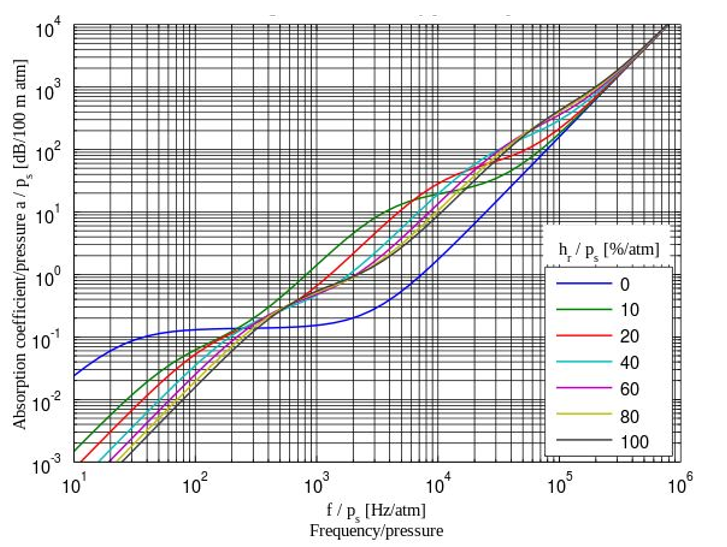
\includegraphics[width= 15cm]{a.png}
\caption[Attenuation of sound at difference frequencies]{Sound absorption coefficient per atmosphere for air at 20 degree Celsius according to relative humidity per atmosphere.\cite{14}}
\label{fig:logo}
\end{figure}


\paragraph{}
The above image \ref{fig:logo} is a graphical display of the attenuation of sound at difference frequencies \cite {5}, which shows that low frequency waves have low absorption coefficient. Therefore, low frequencies are not absorbed well and travel further than high frequencies. This property of infrasound waves can be used  for the acoustic detection of the wave from a greater distance from the source of the sound. The low-frequency sounds used by elephants for long-range communication travel a distance that exceeds 1 km \cite {3}. As mentioned in the section 1.1, this research focuses on detecting elephant infrasonic calls from long distance and localizing them. Detecting and localizing elephants is an essential component of any viable solution to human elephant conflict. Attempts towards acoustic detection and localization of elephants exist in literature. However, due to high cost in infrasonic sensors and complexity in detection of these signals  in noisy environment, no system exists to date, that operation ready in the field.

\paragraph{}
Various types of devices which are capable of capturing infrasonic waves exist and they are mostly used for detecting geographical phenomena such as earthquakes and volcanic eruptions. One such device used by most related research is Infitec Infra 20, which has a sampling rate of 50Hz. This device can be considered as a low cost infra sound recorder compared to other existing devices and this costs US\$ 345 \cite {7}. A significance of this research is the attempt to use a laboratory made sensor system which cost only US\$ 15, which is capable of recording at a sampling rate of 44100 Hz. This sensor system consists of a Panasonic Omnidirectional Back Electret Condenser Microphone \cite{15} (Model WM-64C/WM-64K), LM358 IC for amplifying and a low pass filter\cite{16}.This sensor has the ability to capture infrasonic waves from a lower bound of 0 Hz to an approximate upper bound of 150 Hz.


\paragraph{}
The second research question is based on infrasound localization, which can be done by measuring physical quantities like sound pressure and particle velocity. The best localization technique which is used by nature (Animal sound localization) can be applied to this context in localizing a sound source digitally. Humans as well as most other land-living vertebrates use the time delay between the arrival of a sound wave at each ear to discern the direction of the source \cite {8}. Similarly, localization can be done digitally by calculating the inter-aural time delay  between two microphones lying on a specified distance, which will be further explained in the research methodology. Potential problems include the detection in noisy environment, sparsity and irregularity of elephant call and pattern recognition. These problems will be addressed using advanced digital signal processing techniques and the knowledge based on the existing literature.

\subsection{Scope of the Thesis.}
\paragraph{}
As the final outcome, our intention is to introduce a low cost elephant detecting and localization system specialized for Asian countries using the sensor equipment made in the Sustainable Computing Research Group at University of Colombo School of Computing. In order to achieve the objectives, this thesis will divide our problem of interest in to two parts as localization and pattern recognition. Although they the final outcome should consist of the combine out come of the solutions to this problem for a reducing the complexity this thesis will handle them as two separate problems. 

\begin{flushleft}
\text{This research attempts to:}
\end{flushleft}

\begin{itemize}

\item 	Identify an elephant call in the infrasound range with low latency.
\item 	Localizing an elephant call using the low cost sensors system consisting of a condenser microphone.
\end{itemize}

\paragraph{}
The thesis is organized as follows. Chapter 2 describes related work around the domain and what approaches have been used in infra sound localization, elephant communication, and acoustic detection of the elephants.  In Chapter 3, we have described designs and the methodologies we used in this research. Chapter 4 defines the implementation of the devices, sound localization and the elephant detector. In Chapter 5 we present our results and evaluation of the experiments carried out in both of the above mentioned problems. Chapter 6 used to define future work for our research and to conclude the research.



\newpage
\section{Review of Literature.}
\subsection{Elephant Communication.}
\paragraph{}
Various research types exist in this specific domain. The experiments carried out by Katharine Payne, a researcher in the Bio Acoustics Research Program at the Laboratory of Ornithology at Cornell University, show that elephants use infrasound in communication, which can be considered as the initial steps of all research work on this area. In 1984, she discovered that elephants communicate in low frequencies during her research carried out at the Portland Zoo. Further, her work with William Langbauer, Jr. and Elizabeth Thomas have shown that elephants were indeed making infrasonic calls. Subsequent studies, in association with Joyce Poole, William Langbauer, Cynthia Moss, Russell Charif, Rowan Martin and others, took place in Kenya, Namibia, and Zimbabwe, leading to the conclusion that elephants use their powerful deep calls in long distance communication [6] and elephants make these calls when coordinating family and larger group behaviors, when competing for resources and dominance, as well as when attracting mates and announcing reproduction. Large vocal cords of elephants were able to produce low frequency sound signals considered as rumbles, which were able to travel around 5 kms in distance \cite {6}. It is also revealed that the rumbles audible to human ears, are the harmonic waves created from the infrasonic fundamentals.


\paragraph{}
There have been comparatively less number of study of communication in Asian elephants. Acoustic communication in the Asian elephant by Dr. Shermin de Silva, a  James Smithson Fellow at Smithsonian Conservation Biology Institute, can be considered as a comprehensive study on communication in Asian elephants, which was published in the Behaviour Biological Journal in 2010. She categorized acoustic features into 8 'single' calls, 5 'combination' calls and one possibly unique male call, for a total of at least 14 distinct call types \cite {19}. Her observations and conclusions are based on the data collected at Udawalawa National Park, Sri Lanka during 2007 and 2008. It is mentioned that 7 out of 14 distinct call types (rumble, rev, roar, cry, bark, grunt, husky-cry) are made out of elephants larynx and most of the fundamentals of these calls were found to be infrasonic. While African elephants were the main subjects of considerable amount of existing literature with majority of these focusing on elephant detection in noisy environment; the human elephant conflict is more of a burning issue in South Asian countries like India and Sri Lanka. As a result in 2002, there was an attempt of implementing a sensor system that detects infrasonic calls of elephants in Sri Lanka \cite{13}.

\paragraph{}
Elephant infrasound have not been recorded in wild Asian elephants anywhere in Asia prior to this Sri Lankan research project in in 2002. The prototype introduced by the above research was able to support four infrasound sensors and was capable of standard DSP functions such as archiving and filtering. Sound detection has a long history although it was not specified to elephant infrasound calls. Recent researches have shown that this is possible using a template based or feature based technique. Matched filter method where two spectrograms of the pattern template and the signal are directly mapped is a straightforward mechanism for detecting a pattern in a signal. Although it was optimal when finding the occurrence of a template in a recorded signal it is sub optimal in the presence of complex noise \cite {10}. Therefore, a novel spectro-temporal method for signal enhancement based on the structure tensor \cite {11} was introduced by a group of researchers at University of Vienna, Austria. 

\subsection{Sound Localization.}
\paragraph{}
There are many works related to sound localization using microphones. Many techniques and algorithms have been introduced during past decades to detect the direction of sound emitting source. These are mainly based on the following three types of principles.
\begin{enumerate}
\item Time difference of arrival where the systems measure the difference in time between the signals received by the microphones to localize the sound source.
\item Direction of arrival where the phase difference between the signals is used to locate the sound source \cite {20}.
\item Energy based sound localization where the energy of sound wave decreases when the sound wave propagates in the air. By measuring the sound energy at different sensor locations, one may localize the sound source \cite {21}
\end{enumerate}

\paragraph{}
The most significant technique is the time delay estimation, due to its simplicity and accuracy \cite {22}. Several research works have compared the algorithms such as cross correlation method \cite {23}, phase transform \cite {24} and maximum likelihood estimator \cite {25} used to estimate the time delay. There are instances where they have used two sensors or array of sensors for the localization when number of sensors increases, the mean error generated becomes relatively low \cite {26}.

\paragraph{}
Results of the experiments in the form of simulation results \cite {26} show that all methods were able to estimate the time delay, where the peak position indicates the time delay estimation. However, the Phase Transformation Method  achieved a sharper peak than the other methods, which helps to estimate the real delay time more accurately in the real situation. The maximum likelihood method also achieved a sharp peak. Although cross correlation has the widest peak, it still can estimate the real time delay in the simulation conditions. Since these works can be directly incorporated to elephant call localization, we can guarantee that the accuracy of the localization results can be increased. As a result, we are able to select and use the most convenient and easily implemented method for the localization experiments. The environment of the localization scenario can result in the lagging of sound waves. As elephant localization is done in a forest environment, this is a factor that should be taken in to account. Many works have been done regarding the localization of sound in reverberation environment. The precedence effect describes the phenomenon, whereby echoes are spatially fused to the location of an initial sound, by selectively suppressing the directional information of lagging sounds (echo suppression). Echo suppression is a prerequisite for faithful sound localization in natural environments but its reliability depends on the behavioral context \cite {27}. These works can be integrated with our findings to be produce an accurate infrasonic localization. 

\subsection{Acoustic Detection of Elephants}
\paragraph{}
Although different literature exist with regard to acoustic detection of elephants and infrasound waves, there is no significant attempt towards an economically feasible solution for localizing Asian elephants through the use of infrasound calls, applicable to developing countries like Sri Lanka and India. The review will emphasize the importance towards a research on addressing the above problem. The most comprehensive study on acoustic detection of elephants available right now is \cite{11}. They use a Support Vector Machine for classifying the rumbles after applying the signal enhancement method mentioned above. There are two sound detection approaches mentioned in \cite {11}: template based method and feature based method. In the template based method, in order to find the occurrence of a template it successively matches a given sound example against the audio database. The Matched filter method is a straight forward template based approach, where two spetrograms are directly mapped. Although this method is optimal to find occurrences of the template, it's sub optimal if there are complex noises present in the signal.

\paragraph{}
The next approaches for sound detection are feature based techniques. It introduce an additional layer of abstraction by the features that provide a higher level representation of the sounds. In the \cite{11}, they have developed a feature based technique upon certain acoustic characteristics of elephant rumbles. For avoiding harmonic structure of elephants buried by the noise they apply a structure tensor derived from gradients of the rumble spectrograms and this will be discussed in the Chapter 04. 


\newpage
\section{Design and Methodology.}
\paragraph{}
As mentioned in section 1.4, this research will not produce an ultimate machinery to detect and  localize elephants. Rather, it will be an input to a system of this calibre, which will increase the accuracy and also helps to validate the results of such a system. This research was undertaken in two steps to answer our two research questions.

\paragraph{}
The first phase of the research was mainly focused on the infra sound localization from a relatively large distance and the second phase was on acoustic detection of elephants by processing the sounds recorded using the laboratory made sensors. In this chapter, the designs and the methods that we used to solve our two research questions is explained in detail. The process of the experiments related to infrasonic localization and detection of elephant calls is to be discussed later in this section.

\subsection{Hardware used}

\paragraph{}
One of the objectives of this research is to use low cost and sustainable hardware. In this, we present brief introductions on each commodity and the newly build and engineered hardware by us which will be used in the final outcome and in experiments. 

\paragraph{}
Since we were dealing with infrasound we needed to have a device that is capable of recording infra sound upto 300Hz, which is the upper limit of an elephant call. Although they emit fundamentals at 5Hz-20Hz we needed to record their harmonics to identify the temporal structure of the calls clearly. We have used commodity infrasonic recorder initially and due to it's high cost in large scale deployment scenarios we built a recording module using off the shelf microphones. In section 3.1.1 and 3.2.2 we compared these devices. 

\subsubsection{Infiltec INFRA-20}  

\paragraph{}
Researchers studying lightning activities in the atmosphere and seismic activities also use infrasonic detectors of
various forms. While the devices they use vary in a wide price range, the cheapest device we could identify in the market
is the Infiltec Model INFRA-20 \cite{29}. It costs about USD 300 which is still a significant cost when considering large
scale deployments. It has a sample rate of 50 and a precision of 16 bits. This can be powered by either house current 110-240 VAC or 12 VDC car battery. \cite{29}

\paragraph{}
The INFRA20 electronic noise level is about 20 counts (20 mPa or 60 dB SPL) over the full bandwidth, and this can be measured by cross connecting the ports on the internal differential pressure sensor. The lowest ambient infrasound level over the full bandwidth that we can expect to record with the INFRA20 is about 30 counts (30 mPa or 63.5 dB SPL), typically during the middle of the night when the wind is calm and there are no nearby infrasound sources. The INFRA20 background noise level is low enough so that the microbarom peak at about 0.2 Hz can sometimes be detected above the ambient noise when the wind is calm \cite {29}. The following image is a INFRA20 unit.

\begin{figure}[H]
\centering
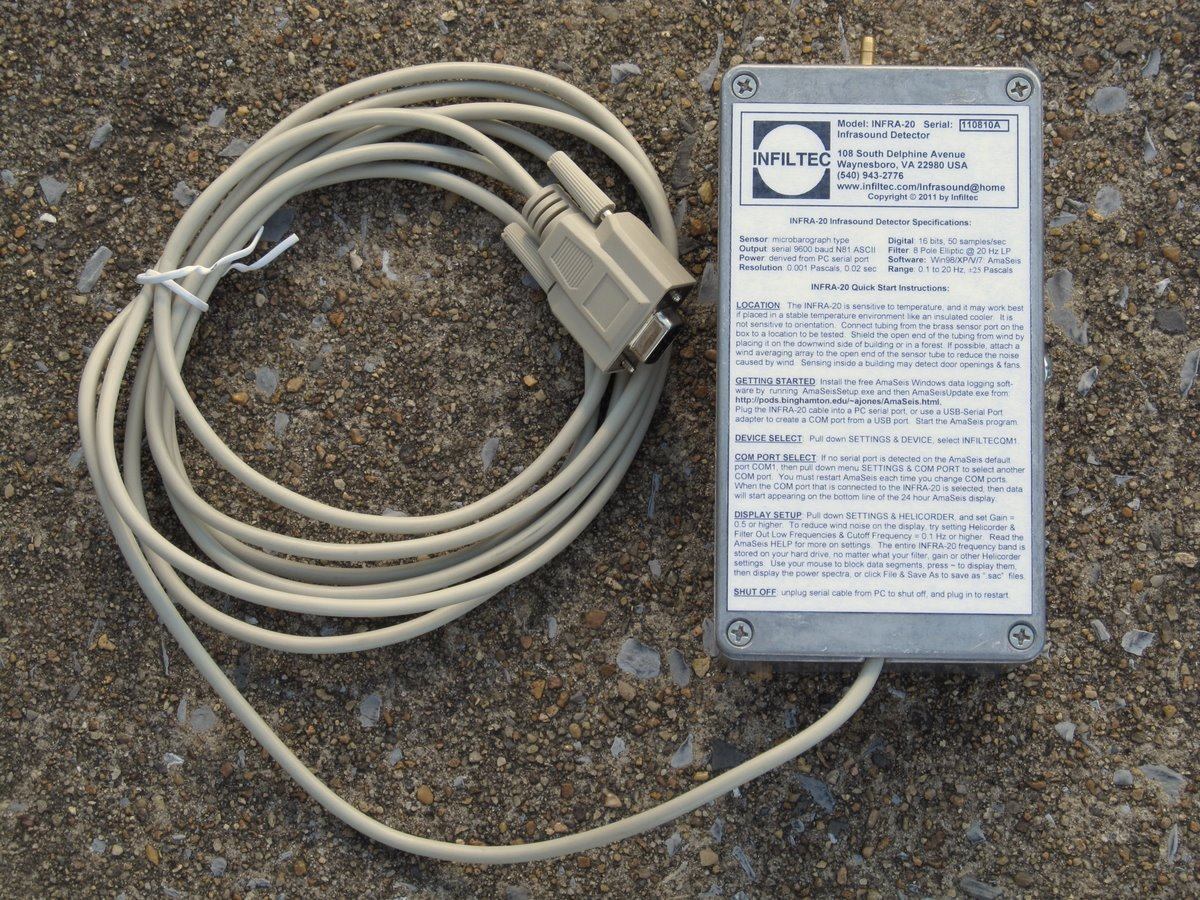
\includegraphics[width=10cm,height=13cm,keepaspectratio]{INFRA_20.jpg}
\caption{Infiltec INFRA-20 device}
\label{d:p12}
\end{figure}


\newpage
\subsubsection{Elocate sensors}

\paragraph{}
In order to localize elephants using infrasonic emissions, it is necessary to have cost effective infrasonic detector systems. Most importantly, since we are deploying them in rural areas of country in large numbers, they need to have a cheap unit cost. Moreover, they should be able to run with minimum maintenance due to the unavailability of technical experts in potential deployment areas. The ability for a rural villager with minimum technical knowledge to set up and run such an elephant localization system in the neighborhood to protect their premises would be a great advantage. The system has to be non-invasive to the elephants to avoid legal barriers of deploying such a system by individuals living in affected areas.

\paragraph{}
To match our needs, we design and implement an infrasonic detector which is called Eloc node. The heart of an Eloc node is a Panasonic WM-61A omnidirectional back electret condenser microphone \cite{15}. Compared to ordinary condenser microphones, this microphone consumes less electric current and is therefore suitable for using in low power devices such as battery-operated embedded systems. An Eloc node consists of such a microphone and a small preamplifier circuitry connected to it inside a sealed plastic container.

\begin{figure}[H]
\centering
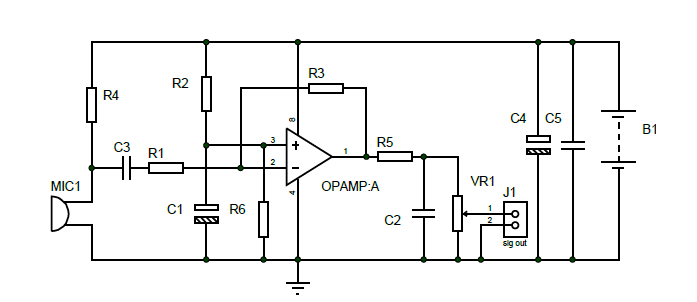
\includegraphics[width=10cm,height=13cm,keepaspectratio]{circuit.png}
\caption[Circuit diagram on an Elocate node]{The pre amplifier schematic used in an Eloc node.
It consists of an operational amplifier in inverting mode and
a low-pass filter. The low-pass filter attenuates frequencies
above 150 Hz.}
\label{image:circuit}
\end{figure}

\paragraph{}
As shown in Figure \ref{image:circuit} , the pre amplifier consists of an operational amplifier in inverting mode and a low-pass filter. The low-pass filter attenuates frequencies are above 150 Hz since we are interested only in infrasonic frequency components. Eloc nodes get power from a 9V battery attached to the plastic container. This complete unit draws a current less than 50mA from the battery when the microphone is active. Hence Eloc nodes could be powered by solar cells to avoid the need of replacing batteries once deployed in the field. The output of the Eloc nodes is an analog signal that we can sample directly using a suitable analog-to-digital converter before sending it over a wireless network for processing in the server side. For the experimental purposes we connect it directly to the audio input port of a computer for processing on-site.

\subsubsection{Subwoofer and Amplifier}
\paragraph{}
We are using a full range speaker as the infrasonic emitter with the help of an amplifier. This amplifier consumes 500 watts and designed for amplifying sub woofers.



\newpage

\subsection{Localization of the infra sound}
\paragraph{}
Localization in this context is locating the infra sound emitting source. Localization of objects with tags which emits electromagnetic waves is a well studied problem with various localization techniques. Due to the maturity of such techniques,
the most obvious way of locating living objects such as humans and animals is tagging them with wireless devices. Radio collars placed on elephants is one good example of such an application \cite{32}. However placing wireless devices on wild animals is intrusive to the natural behavior of the animals and such techniques are frowned upon by animal conversationalists. In addition, the difficulties in physically reaching elephants to attach these devices also make this a cumbersome solution.

\paragraph{}
Our objective is to localize elephants by detecting their infrasonic emissions using Eloc nodes. Wang et al. have studied the use of acoustic sensor networks to passively localize wild animals \cite{33}. Our focus, is to use the infrasonic emissions from Asian elephants to detect and localize elephants. While many different sound localization methods are available in the literature, we use a simple technique based on Time Difference Of Arrival (TDOA) to locate infrasonic sources. The basis of this technique is presented by Kim et al. \cite{34} for localizing humans using the sounds they make. Due to the fact that those are audible sounds, their work considers capturing audible frequencies within close range mostly in indoor environments. In contrast, we consider a limited bandwidth in the infrasonic range which is heavily affected by natural low frequency noise sources such
as the wind. Reasons for using TDOA are it's implementation simplicity and ability to deploy in low powered computing devices. 

\subsubsection{Time delay estimation}
\paragraph{}
Time delay estimation is determined by the relative time difference of arrival between signals received by different sensors. Phase shift of each signal is measured relative to the other signal and this is used to calculate the time delay of arrival. This time delay is calculated using cross correlation technique which will be explained in the section below. In this scenario time delay estimation is done using the infrasonic signals received by  two Elocate sensors placed few distance away from each other. \ref{sinewave} will show how a sinusoid signal will be recorded by two Elcoate sensors. 

\begin{figure}[H]
\centering
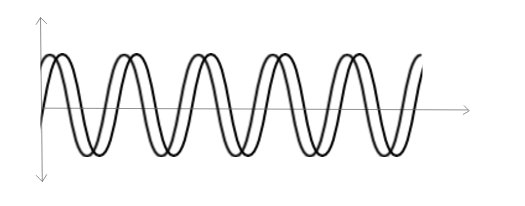
\includegraphics[width=100mm,height=50mm]{sinewave.png}
\caption{Sine wave in a the time domain}
\label{sinewave}
\end{figure}

\paragraph{}
This time delay is used to used to calculate the angle between the sensors and the sound emitting source. And this can be used for the localization of the source. 

\subsubsection{Cross correlation}

\paragraph{}
Signal data recorded by two sensors is in the form of digital. Therefore these two signals are in the form of array having the normalized amplitude at each sample. Cross correlation come into play when we are calculating the time delay of arrival using these two arrays. Cross-correlation measure the similarity of two signals as a function of the displacement of one relative to the other. A signal recorded from one sensor is displaced relative to the other signal recorded from the remaining sensor and sliding inner product is taken. The below figure \ref{crosscor} show how one signal is slide relative to the other signal.

\begin{figure}[H]
\centering
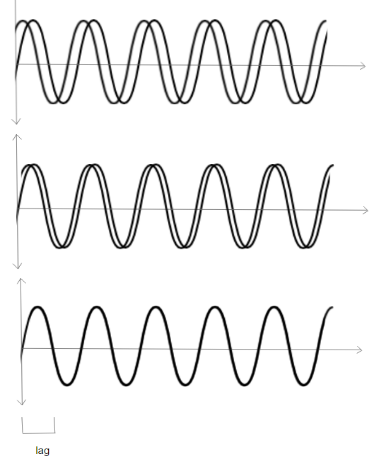
\includegraphics[width=80mm,height=150mm]{crosscor.png}
\caption{Correlation process}
\label{crosscor}
\end{figure}

\paragraph{}
Slided amount along the time axis at the maximum sum of product gives the time delay of arrival. Because the maximum sum of product gives the location where the signals correlate each other. Since these two signals are not identical and affected by different type of noise and other factors this maximum correlation gives a fair trade off for the time delay of arrival. One limitation of this method is that, since these signals are periodic, after the first maximum correlation, at each and every 180 degree shift an another maximum correlation occurs. Therefore the maximum time delay of arrival should not give a phase different more than 180 degree. This delay is depend on the distance between the two sensors and in infrasonic recording scenario this distance should be determined according to the signal wave length that we are going to localize. 

\paragraph{}
Asian elephants communication range is 14Hz to 24Hz \cite{2}. Since our Elocate nodes start cutting high frequencies at 150Hz maximum harmonic frequency of 20Hz fundamental is 120Hz. So we select 120Hz as the maximum record-able frequency. This selection enables us to use frequencies below 120 Hz for the localization which includes a number of higher harmonics in addition to the fundamental frequency components of the elephants in the infrasonic range. If we assume that the average temperature is 30 $^{\circ}$ Celcius velocity of the sound will be 350 m/s. So from equation (1).

\begin{equation}
v=f\lambda
\end{equation}
\begin{equation}
\lambda=v/f
\end{equation}
\begin{equation}
\lambda=350/120
\end{equation}
\begin{equation}
\lambda=2.916
\end{equation}

From the above calculation we select 3 meters as the distance between the Eloc nodes which is roughly the wavelength of the frequency 120 Hz under the atmospheric temperature of 30 $^{\circ}$ C to avoid capturing signals with a phase difference than 180 $^{\circ}$.


\subsubsection{Estimation of the sound direction}

\begin{figure}[H]
\centering
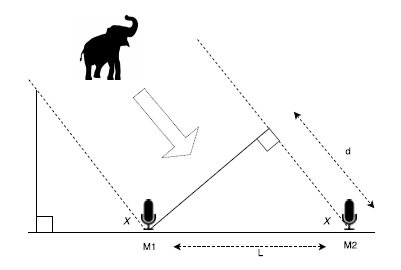
\includegraphics[width=140mm,height=100mm]{direction.png}
\caption[Localization scenario]{Basic setup to calculate the direction of an infrasonic
source using two Eloc nodes. The node pair is placed
within a constant distance to each other and continuously
capture data in a time synchronized manner in order to localize
the source using time difference of arrival.}
\label{direction}
\end{figure}

\paragraph{}
Figure \ref{direction} illustrates the basic setup to calculate the direction to an infrasonic source using two Eloc nodes. The infrasonic wavefront from the source arrives at the microphone M1 and then passes through it to the microphone M2. We take the distance the wavefront travel from M1 to M2 is d as illustrated in the figure \ref{direction} and the time delay for this journey is taken as D seconds. The same signal captured by M1 is captured by M2 after the D time delay. This time delay of arrival can be estimated by taking the cross correlation of the signals captured by M1 and M2. The lag towards the peak in the cross correlation graph indicates the phase shift between the two signals due to the delay D the infrasonic waves took to travel from the microphone M1 to the microphone M2. This phase shift can be measured as a number of samples, n. If the sampling rate at each microphone is f , we can have a representation of the time delay D as follows. 

\begin{equation}
D=n/f
\end{equation}

\paragraph{}
We can deduce an equation for the time delay D, according to the geometry in Figure \ref{direction}, as follows. The speed of
sound is taken as Vsound and the distance between the two microphones is L which are known values. The angle of infrasonic
waves arriving at the line connecting two microphones is x in degrees.

\begin{equation}
D = d/ Vsound = L Cos x/ Vsound
\end{equation}

\paragraph{}
Based on the Equations 5 and 6, we can calculate the angle x as follows.

\begin{equation}
x=\cos ^{ - 1} (nVsound/Lf)
\end{equation}

\paragraph{}
Equation 7 shows that when we know the sample lag between
the same sound captured by two Eloc nodes, we can
directly calculate the angle to the elephants location from the
node pair. However, when using a recorded sound clip as a
whole for the correlation calculation, different noise sources
that affected each Eloc node lower the accuracy of the final
result. To minimize such effects, we need multiple sound
clips from the elephant while it is in the same location over
the time period of capturing the sound. Due to the difficulty
of capturing multiple sound clips in such a way, we break a
single sound clip into windows so that we can consider each sample window as a separate data input for the correlation
calculation.

\begin{figure}[H]
\centering
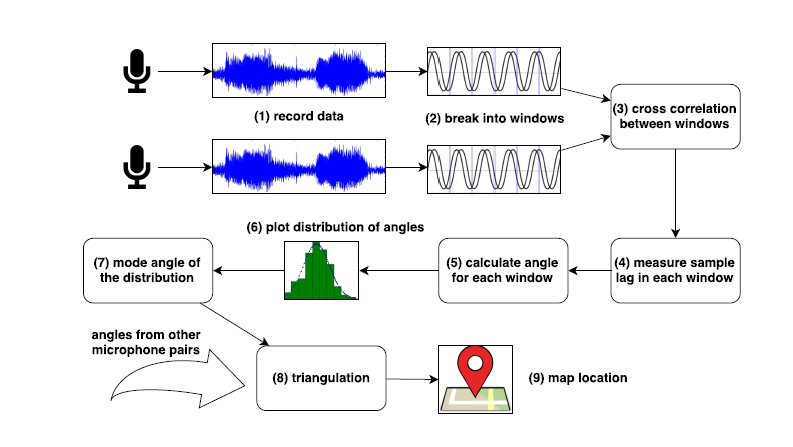
\includegraphics[width= \textwidth]{crosscor_implementation.png}
\caption[Process of calculating the location of an elephan]{Process of calculating the location of an elephant.
A pair of Eloc nodes capture elephant sounds which we
break into windows, cross-correlate, calculated the sample
lag and finally use it as an input for the angle calculation.}
\label{crosscor_implementation}
\end{figure}

\paragraph{}
Figure \ref{crosscor_implementation} illustrates the complete process of locating an elephant using the infrasonic data. In the first step, two Eloc nodes capture infrasonic data in a time synchronized manner and we sample and quantize their output as the first step. Secondly, we break the data sets of the two channels into multiple windows of equal sizes to get multiple data samples from the original recordings. Then we take each corresponding window pair from the two channels and calculate
the cross correlation between them (Step 3). The number of sample points (i.e: lag) to the peak of the cross correlation
is the phase shift n in the Equation 7 that we compute in the fourth step. Using this value, we calculate the angle to the
infrasonic source for each sample window in Step 5.

\paragraph{}
Since we have multiple windows, we get multiple angles to the infrasonic source which may not necessarily be the
same value due to the noise in our recorded data. As Step 6 of Figure \ref{crosscor_implementation}, we plot the distribution of calculated angles for multiple windows for a known sound source. In the next step, we take the statistical mode of the distribution as the most representative angle that represents the actual angle towards the sound source. Our eventual goal is to deploy multiple pairs of Eloc nodes. In Step 8 we can then perform triangulation based on the angles calculated using each node pair to compute the position of the elephant in Step 9.

\paragraph{}
According to Equation 7 the angle calculation depends on the speed of sound, distance between the Eloc nodes, sampling
rate of the nodes, and the lag taken from the cross correlation. We can consider all the parameters as constants
except the lag, n, towards the cross correlation peak. The calculated angle is a non-linear function of n. That means, to
get the same change of degrees in the calculated angle, the required change in sample lag will be different from angle to
angle. Since this phenomena has an important effect on the errors we observed in real world experiments, we analyze the
behavior of angle calculation.

\subsubsection{Estimation of the error}

\paragraph{}
Minimum difference in the sample lag that we can measure depends on the sampling rate of the analogto-
digital conversion (ADC) on the connected computer. For a sampling rate of f , the minimum resolution of time measurement
we can have is (+/-)1= f . Since the sample lag n in Equation 7 has the same resolution, the error in n becomes
(+/-)1= f . We analyze the propagation of this error to the calculated angle as follows.

\paragraph{}
According to the error theory \cite{35}, the error, \Delta x, propagated to the calculated angle x is,

\begin{figure}[H]
\centering
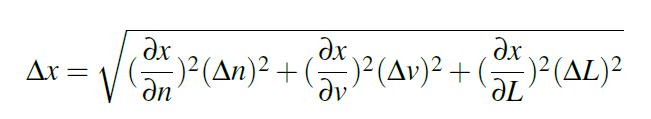
\includegraphics[width=100mm,height=20mm]{error.png}
\end{figure}

where, \Delta n, \Delta v, and \Delta L are the the measurement errors in the lag, speed of sound and the distance between Eloc nodes. Under the assumption that the speed of sound and the distance between the two Eloc are constants, this simplifies to,

\begin{figure}[H]
\centering
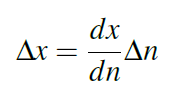
\includegraphics[width=30mm,height=15mm]{error1.png}
\end{figure}

\paragraph{}
From equation 7,

\begin{figure}[H]
\centering
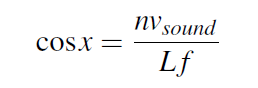
\includegraphics[width=35mm,height=15mm]{error2.png}
\end{figure}

\paragraph{}
We differentiate it by n,

\begin{figure}[H]
\centering
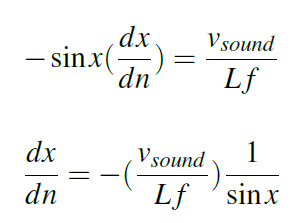
\includegraphics[width=45mm,height=35mm]{error3.png}
\end{figure}

\paragraph{}
During the time period of the experiments, we assume that the speed of sound (Vsound ), the distance between the two
microphones (L) and the sampling rate of the microphones ( f ) are constants. Therefore,

\begin{figure}[H]
\centering
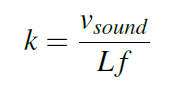
\includegraphics[width=30mm,height=15mm]{error4.png}
\end{figure}

\paragraph{}
So by substituting the constant,

\begin{equation}
\frac{dx}{dn}=-k(\frac{1}{sin x})
\end{equation}

\subsection{Acoustic detection of the elephant calls}
\paragraph{}
Due to the fact that the elephants communicate with each other by low-frequency sounds, which travel distances of several kilometers acoustic detection of elephants by their calls has become a promising approach. In this section we discuss the methodology of automating the detection of recorded elephant calls in a machine learning approach. Major challenges that we faced in the process of automating the elephant call detection are the large variety of uncontrollable noises from wind, rain, cars and airplanes, and sparsity and irregularity of elephant calls, which makes it difficult to predict the occurrence of a call. We employ an image processing based signal filtering mechanism to filter out this noise based on the work of \cite{11}.
\paragraph{}
Initially, we train the model without any signal enhancement or noise filtering mechanism. And then the spectro temporal enchacment proposed by \cite{11} is applied and results are compared. We are dealing with a signal data set which basically are audio clips in time domain. The signal consist of the mean amplitude of each sample and all other information such as frequency and wavelength can be extracted using it. To a classifier these raw data doesn't make any sense. Main objective of this kind of classification is clearly distinguish the waves of elephant calls and waves without elephant calls. So that the all the features that distinguish elephant calls from other sounds should be extracted to feed into the classifier. So in the first step features are extracted from the waves.

\subsubsection{Feature extraction}
\paragraph{}
The first step in automatic elephant call detection is to extract features i.e. identify the components of the audio signals that are good for detecting the elephant vocal contents and discarding all the other stuff. Feature extraction is the process of computing a compact compact numerical representation that can be categorize a segment of audio. Naturally this done in human ears by filtering out according to the shape of the vocal tract including tongue, teeth etc. The same technique is modeled mathematically to filter out the unnecessary things mentioned above. 

\begin{figure}[H]
\centering
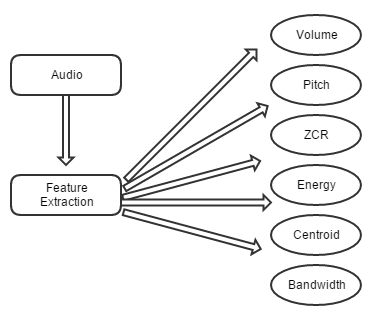
\includegraphics[width=12cm,height=15cm,keepaspectratio]{feature_extraction.png}
\caption{Overview of the feature extraction.}
\label{feature_extraction}
\end{figure}

\paragraph{}
Apart from the acoustic qualities global temporal, energy, spectral shape and harmonic  are some of the features that can be extracted in order to identify the elephant calls. Extracting this features reduces the complexity of the machine learning model by the reduction of the dimension of the input data. There are few techniques that is used to extract features from audio widely used in speech recognition of human and here we adopt such a technique according to our requirement.
 
\subsubsection{Adopting Mel Frequency Cepstral Coefficients}
\paragraph{}
Mel Frequency Cepstral Coefficient (MFCC) is the widely used audio feature extraction method in human speech processing domain \cite{36}. It was introduced by Davis Mermelstein in the 1980's and have been the state of the art feature extracting mechanism since. Before MFCC was introduced, feature extraction was done by Linear Prediction Coefficients and Linear Prediction Cepstral Coefficients. In the section we will be discussing how MFCC was adopted to extract features from the data set used to train the machine learning model.

\paragraph{}
MFCC is done in following steps.

\begin{enumerate}
  \item Framing of the signal into small frames.
  \item Calculation of the periodogram estinate of the power spectogram for each frame.
  \item Applying mel filterbank to the power spectrum and summing up all the energies in each filter.
  \item Getting the Logarithmic value of filter bank energies.
  \item Getting the Discrete Cosine Transformation (DCT) of the log filter bank energies.
  \item Keep the coefficients 2-13 and discard the rest.
\end{enumerate}

An audio signal is frequency subjected to changes in the amplitude. So we assume that on short time scale the amplitude is statically stationary. Therefore in the first step we frame the audio into 20-40 frames. If the frame is much shorter then we cant reliable spectral estimate, if it is longer the signal changes too much throughout the frame. Next we calculate the power spectrum of each frame. This is motivated by the human cochlea which vibrates at different spots depending on the frequency of the incoming sounds. Depending on the location in the cochlea that vibrates, different nerves fire informing the brain that certain frequencies are present. Since we are interested in elephant auditory system we change the MFCC parameters accordingly. So we use more generalized method introduced by Greenwood. This requires the definition of three species specific parameters namely the hearing range of the animal species which is 10Hz to 10000Hz and a constant k=0.88  that represents the nature of the cochlea as in \cite {37}. 

\paragraph{}
Power spectrum estimate still contains lot unnecessary information for automatic elephant call detection. The cochlea can not discern the difference between two closely spaced frequencies. Due this reason we take clumps of periodogram bins and add them up to get an idea of how much energy exists in various frequency regions. This is done by Mel filter bank which initially indicates how much energy exist near 0 Hertz in first filter. And as the frequency increases these filters get wide and become less concerned about variations. We are only interested in how much energy occur in each frequency level and Mel scale can be used to get the spacing of filter banks. The Mel scale relates perceived frequency, or pitch, of a pure tone to its actual measured frequency by the following functions.

Conversion of frequency to Mel Scale 
\begin{equation}
M(f) = 1125 ln (1+f/700)
\end{equation}

Conversion of Mel Scale to frequency
\begin{equation}
M^{-1}(m) = 700 exp((m/1125)-1)
\end{equation} 

\paragraph{}
After applying filters, we take the logarithm of them. This allows us to use cepstral mean subtraction, which is a channel normalization technique. Final step is to calculate the Discrete Cosine Transformation (DCT) of the log filter bank energies. This is performed due to two reasons. Because the filter banks are all overlapping and the filter bank energies are quite correlated with each other. We drop 14 of the DCT coefficients and only 12 is kept because the higher DCT coefficients represent fast changes in the filter bank and due to that ASR degrades its performance. Dropping some of them make a small improvement.

\subsubsection{Signal enhancement}
\begin{figure}[H]
\centering
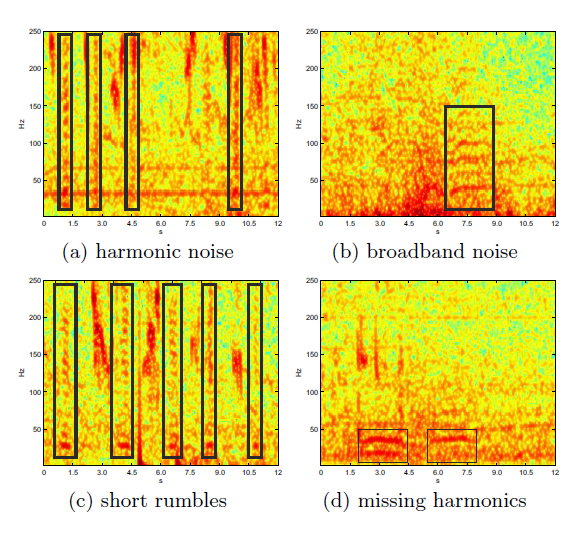
\includegraphics[width=12cm,height=15cm,keepaspectratio]{SNR.png}
\caption{Rumbles with different interfering noise
sources.}
\label{SNR}
\end{figure}
\paragraph{}
Natural sounds from wind and rain, other artificial low frequency sounds from sources like engines generate a broadband noise  reduces the signal to noise ration. Figure \ref{SNR} shows how the background noise mask the harmonic structures and make them hard to detect. Signal enchantment emphasize the spectral structure of rumbles to facilitate the automated detection. Spectral structure of rumbles extend in frequency as well as in temporal dimension. 

\paragraph{}
We will be applying the signal enhancement proposed by \cite{11}, as it is. In that work they have proposed an image processing mechanism to enhance the frequency contours and spectral peaks. This is similar to the detection of edges and corners in an image. Structure tensor is a powerful method for the detection of such structures \cite{38}. So in order to increase the signal-to-noise-ratio and to enhance the spectrotemporal structures  we apply the structure tensor according to the work of \cite{11}. 

\paragraph{}
Signal enhancement process is done in the following steps.

\begin{enumerate}
  \item Form the spectrogram of the signal.
  \item Applying the structure tensor to the spectrogram to enhance spectrotemporal
structures and to increase the signal-to-noise ratio.
  \item To make the tensor more robust, the gradients are first smoothed along the time and frequency axis by a
two dimensional Gaussian filter.
  \item Computation of the coherence of each tensor which is a combined measure that provides the amount and the type of structure in a given position.
  \item Applying the coherence as a weighting filter to the spectrogram.
\end{enumerate}

\paragraph{}
The above enhancement process is introduced by the authors in \cite{11} and it discussed in details in their publication.

\subsubsection{Classification using Support Vector Machine}
\paragraph{}
In this section we will be discussing on our classification model and advantages of our choice over other classification models. Some of the popular pattern recognition methods are Hidden Markov Models (HMM), Support Vector Machines (SVMs), Gaussian Mixture Models,(GMM) and Artificial Neural Networks (ANN). What we are trying to classify are elephant rumbles and other sounds. So our objective is to label our audio signals as rumbles and non rumbles.  

\paragraph{}
In the present day SVM paradigm has proved highly successful classification tasks \cite{39}. SVM discriminates the data by creating boundaries between classes instead of estimating the class conditional densities. And also it need considerably less data to perform a accurate classification task. There for we consider SVM as a comprehensive technique to classify our data as rumbles and non rumbles. In fact, SVM has alread used for sound classification in \cite{11} with a true positive rumble detection acuracy of 92\% and in \cite{40} 94 \% accuracy in multiclass sound classification. 

\paragraph{}
SVM is trained using a data set consisted of rumbles and non rumbles. Detailed description of the dataset we used is in the chapter "Result and Evaluation". Each clip is trimmed into 2 seconds windows in order to facilitate the feature extraction process with less computational power, which also affect the training and detection performance. This time was decided by dry running the feature extraction programs on the particular hardware that we are going to deploy. Then these aggregated features extracted from the sound signals are used in the training process.



\newpage
\section{Implementation.}
In this chapter we will be discussing about implementation process of the Elocate nodes, localization and automated acoustic detection system based on machine learning.
\subsection{Implementation of Elocate nodes}
\paragraph{}
Section 3.1.2 consists of the architecture and design of the Elocate nodes and in here we will be discussing about the implementation constraints. 

\begin{figure}[H]
\centering
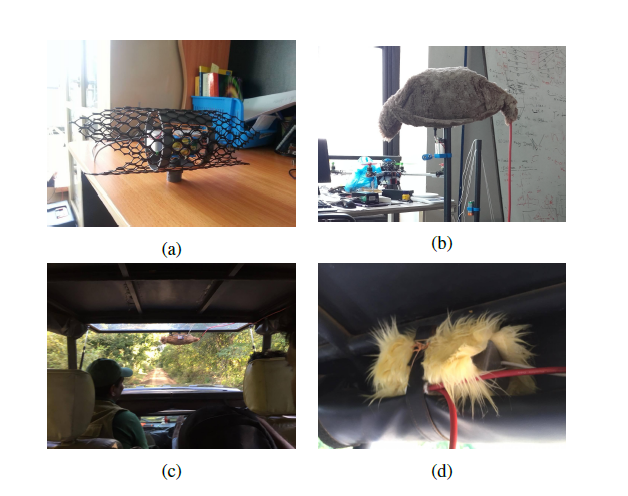
\includegraphics[width=12cm,height=15cm,keepaspectratio]{eloc_implementation.png}
\caption[Implementation of an Elocate node]{(a) The microphone together with pre-amp circuitry
is placed inside a sealed plastic box and then placed
inside the wire-frame with shock mounting. (b) This wireframe
was covered with a soft material to cancel wind noise.
In (c) and (d), two of these microphones are mounted in
front and back of a vehicle for field experiments.}
\label{figure:eloc}
\end{figure}

\paragraph{}
Since we are interested in low frequencies, the noise imposed by the wind plays an important role. Initial experiments indicated that the Eloc nodes are unable to detect low frequency sources since they are submerged under the wind noise floor. Therefore we design and built a wind barrier around the microphones to protect them from wind noise as shown in Figure \ref{figure:eloc}. This wind barrier consists of a wireframe with a soft material attached to it. An Eloc node is placed inside the wireframe using a vibration-proof mounting. We used different soft materials for the fur layer on the wireframe as well as several shapes for the wire frame to identify the most appropriate combination. The selected fur layer consists of a cheap artificial fur material we found off the shelf. Detailed comparison of the Eloc node with the INFRA20 will be in the Vhapter 5.


\subsection{Localization}

\subsubsection{Estimation of the direction}

\begin{figure}[H]
\centering
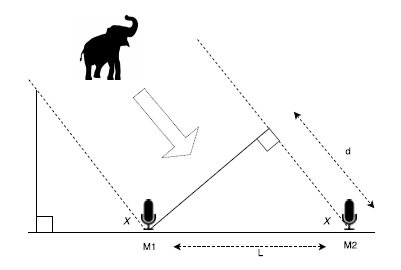
\includegraphics[width=100mm,height=80mm]{direction.png}
\label{direction1}
\end{figure}
\paragraph{}

This was implemented using Python and Matlab for different experiments under deployment environments. This estimation gives a angle , precisely a distribution of angles calculated in each window. Default windows size used is 10000 samples. At this phase the audio recorded is the input to the angle (x in the above diagram) calculation function with the parameters of distance between two Elocate nodes, sample rate and velocity of the sound. The audio should be a two channel audio consist of data from two Elcoate nodes and recorded in 16 bit wave format. A window from first signal is cross-correlated with the corresponding window in second signal and the lag will be calculated. As mentioned in the Methodology this lag is then used to calculate the angle x in the above figure. This will be repeated for each and every window and an angle calculated from each window is stored in an array. If an abnormal result was generated by a noise it will be dropped if the sine value of it is greater than 1. Following code snippet shows this implementation in Python.

\begin{lstlisting}[language=Python]
#filename , sampel rate, distance between two nodes, 
velocity of sound
def getAngle(fi,fs,d,vs):   
    fs, data = wavfile.read(fi)
    data=data.astype('float64')
    data=data.T/32767
    s1=data[0]
    s2=data[1]
    limit=len(data[0])
    fs = 44100
    start_window = 1
    end_window = 10000
    window = 10000
    total = 0
    arr=[]
    while(end_window<limit):
        s1=data[0][start_window:end_window]
        s2=data[1][start_window:end_window]
        xcor=np.correlate(s1,s2,'full')
        m=max(xcor)
        im=np.argmax(xcor)
        start_window = start_window + window
        end_window = end_window + window
        deference = abs(im - window)
        ang = deference*vs/fs/d
        if(ang<=1):
            angle=np.arcsin(ang)
            arr.append(math.degrees(angle))
    plt.hist(arr)
    plt.show()

    return(arr)
\end{lstlisting}

\paragraph{}
For importing wave files wavefile module from Scipy is used and Correlate from Numpy is used for cross-correlation. Matplotlib is used to visualize calculated angles for each window in a particular wave file in a histogram. 

\subsubsection{Sparse Fast Fourier Transform}
\paragraph{}
This was implemented in order to ensure that we receive intended frequency of sound signals. We use Matlab Spectrogram to transfer time domain signal to the frequency domain and calculate the number of samples from each frequency in the input signal. And then the extracted data is visualized in a line chart, mentioning the frequency in X axis and number of samples in the Y axis. Matlab implementation of the SFFT program is given below.

\begin{lstlisting}[language=Matlab]
function [s p] = sfft(data,frnge,sr)
[r c] = size(data);
if(c == 1)
    data = data';
end
ss = spectrogram(data,length(data),length(data)-1,frnge,sr);
s = abs(ss);
p = (angle(ss));
if(pl == true)
    plot(frnge,s);
    title('frequency');
end
end
\end{lstlisting}
\paragraph{}
Parameters of this function are a single channel audio, frequency range that we need to observe and the sample rate. Figure \ref{figure:sfft_output} show the output graph of the above function.

\begin{figure}[H]
\centering
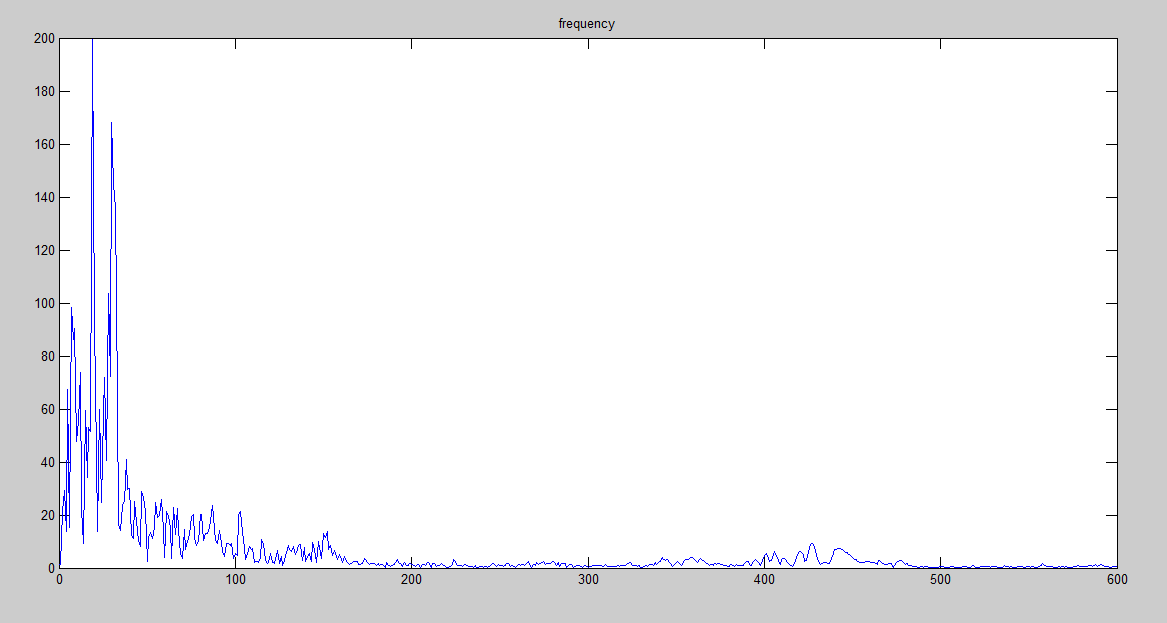
\includegraphics[width=12cm,height=15cm,keepaspectratio]{sfft_output.png}
\caption{Output of the SFT}
\label{figure:sfft_output}
\end{figure}



\subsection{Pattern recognition of the rumbles}
This was implemented in Python 2.7,by considering the fators regarding deployment environment. This module is separated from the above localization module and implemented with minimum inter dependencies which allows this to deploy in a server side environment or in a device with a low power computing board. The pattern recognition module is further broken down into smaller components like Feature extraction, Signal enhancement, Training and Testing. Detailed description of the implementation of each component will be discussed in this sub section.  
\subsubsection{Signal enhancement}
We employ the signal enhancement implemented by the aurthors in \cite{11}. And the implementation is in the appendix A.
 
\subsubsection{Feature extraction}
\paragraph{}
MFCC implementation of Python Speech Features (PSF) was used in feature extraction. Default frequency range of the library was shifted down where maximum frequency will be 300Hz which is suitable for elephant range.

\begin{lstlisting}[language=Python]
from python_speech_features import mfcc
from python_speech_features import logfbank
import scipy.io.wavfile as wav
\end{lstlisting}

\paragraph{}
As shown in the above code fragment MFCC, Logfbank was imported from PSF where MFCC was used to extract cepstral coefficients and Logbank was used to get the logarithmic filters. Signal was imported as a wave file using Scipy wavefile module. This imported signal will be a Numpy array consisting of 16 bit integers.

\begin{lstlisting}[language=Python]
def extract_features(wavefile,winlen):
    (rate,sig) = wav.read(wavefile)
    data=sig.T
    #checking the audio is dual channel or single
    if(len(data)==2):
        mfcc_feat = mfcc(data[0],rate,winlen,winstep=1,highfreq=300)
    else:
        mfcc_feat = mfcc(data.T,rate,winlen,winstep=1,highfreq=300)
        
    return mfcc_feat
\end{lstlisting}

\paragraph{}
The above function accept an audio signal (Single channel or dual channel) and a window length (which will be the smallest unit) to process feature extraction. And this will return a feature vector consist of 13 features which described in the Chapter 3. 


\subsubsection{Spectrogram visualization}

\paragraph{}
Spectrogram visualizer was implemented to identify the rumble patterns visually in the field experiments. Apart from the Python implementation of the spectrogram visualizer Matlab and Audacity was used to analyze the data visually. Implementation of the spectrogram visualizing function is give below.

\begin{lstlisting}[language=Python]
def plotstft(audiopath, binsize=2**10, plotpath=None, 
	colormap="jet"):
    samplerate, samples = wav.read(audiopath)
    s = stft(samples, binsize)
    sshow, freq = logscale_spec(s, factor=1.0, sr=samplerate)
    ims = 20.*np.log10(np.abs(sshow)/10e-6) # amplitude to decibel
    timebins, freqbins = np.shape(ims)
    plt.figure(figsize=(15, 7.5))
    plt.imshow(np.transpose(ims), origin="lower", aspect="auto", 
    cmap=colormap, interpolation="none")
    plt.colorbar()
    plt.xlabel("time (s)")
    plt.ylabel("frequency (hz)")
    plt.xlim([0, timebins-1])
    plt.ylim([0, freqbins])
    xlocs = np.float32(np.linspace(0, timebins-1, 5))
    
    plt.xticks(xlocs, ["%.02f" % l for l in 
    ((xlocs*len(samples)/timebins)+(0.5*binsize))/samplerate])
    
    ylocs = np.int16(np.round(np.linspace(0, freqbins-1, 10)))
    plt.yticks(ylocs, ["%.02f" % freq[i] for i in ylocs])
    
    if plotpath:
        plt.savefig(plotpath, bbox_inches="tight")
    else:
        plt.show()
        
    plt.clf()
\end{lstlisting}


\newpage
\subsubsection{SVM model}
SVM implementation of the Python Scikit-Learn was used in our model. Scikit-learn provide a range of supervised and unsupervised learning algorithms via a consistent interface in Python \cite{41} . It is licensed under a permissive simplified BSD license and is distributed under many Linux distributions, for academic and commercial use.In our scenario, extracted features from the negative and positive data set, which are rumbles and non rumbles are used to train the model. As mentioned in the methodology each input signal is split into 2 seconds windows and every window from a positive data is labeled as '1' which indicates positive and every window from a negative data is labeled as '0' which indicates negative. Given below is the script used for the training.

\begin{lstlisting}[language=Python]
negative_files=listdir('./Negative')
positive_files=listdir('./Positive')

postive_features=[]
negative_features=[]
y=[]
for fil in positive_files:
    feature_vector=extract_features('Positive/'+fil,1)
    for f in feature_vector:
        postive_features.append(f)
        y.append(1)
for fil in negative_files:
    feature_vector=extract_features('Negative/'+fil,1)
    for f in feature_vector:
        negative_features.append(f)
        y.append(0)

x=postive_features+negative_features
clf = svm.SVC()
clf.fit(x, y)


#Saving the model
from sklearn.externals import joblib
joblib.dump(clf, 'Model/model.pkl')
\end{lstlisting}

\paragraph{}
This script read all the files in the Negative directory and Positive directory and label them accordingly. For each audio clip and each window, the feature extraction function will output 13 dimension array consist of the output of the DCT. This is considered as a input data to the SVM and each array will be labeled as '1' or '0'. After the training process, this trained object will be serialized into the model directory and can be used for the detection purposes.

\subsubsection{Testing model}
\paragraph{}
Testing model use the serialized trained SVM object to test the detector. When we input a directory with all the testing data following script will output the result for each signal data.  
\begin{lstlisting}[language=Python]
def test(ffile):
    clf = joblib.load('Model/model.pkl')
    feature_vector=extract_features(ffile,1)
    
    return clf.predict(feature_vector)

\end{lstlisting}





\newpage
\section{Results and Evaluation.}
\paragraph{}
In this section we are discussing about experiments we conducted in the process of answering our two research questions, their results and evaluation. In order to address to the two research questions the experiments and data collecting, on infra sound localization and elephant rumble detection were performed during period of the research. Further we have conducted some experiments to evaluate our Elocate sensors against existing infra sound recorders.

\subsection{Infiltec INFRA-20 vs Eloc Nodes}
\paragraph{}
The microphone manufacturer has specified a sensitivity range between 20 Hz and 20 kHz. As discussed in the literature review, acoustic calls of Asian elephants have, however, fundamental frequency components between 14 Hz and 24 Hz \cite{30}. To evaluate the usability of the microphone for low audio frequencies, we conducted an experiment where we emit a chirp from 10 Hz to 100 Hz using a subwoofer. \cite{30} shows that subwoofers can replay elephant sounds that include fundamental frequency components in the infrasonic range with sufficient output power to emulate a real elephant. Figure \ref{infiltec:eloc} shows that the microphone is sensitive to much lower frequencies than 14 Hz and hence, can be used for the task at hand. Meanwhile, Figure \ref{infiltec:eloc2} illustrates the variation of sensitivity of an Eloc node with the distance to an infrasonic source. The figure \ref{infiltec:eloc2} shows that Eloc nodes outperform the expensive Infiltec Model INFRA-20 device at all distances.

\begin{figure}[H]
\centering
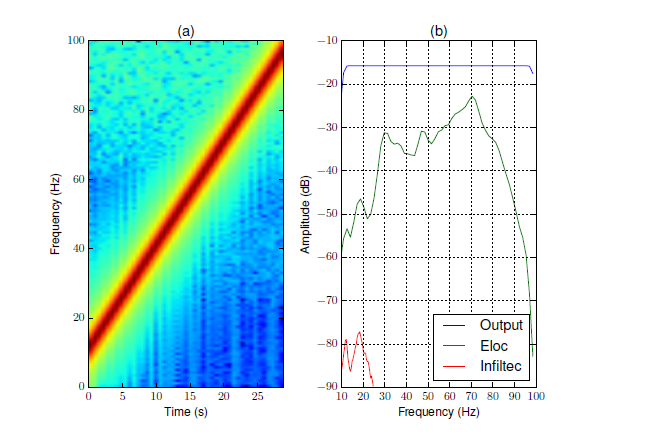
\includegraphics[width=10cm,height=13cm,keepaspectratio]{eloc_vs_infiltec.png}
\caption[Sensitivity comparison of the microphones]{Sensitivity comparison of the microphones for different
frequencies. The spectrogram (a) shows the played
chirp from 10 Hz to 100 Hz and the graph (b) shows the received
power by an Eloc node and an Infiltec device. Eloc
node is sensitive even to much higher frequencies above the
infrasonic range.}
\label{infiltec:eloc}
\end{figure}

\begin{figure}[H]
\centering
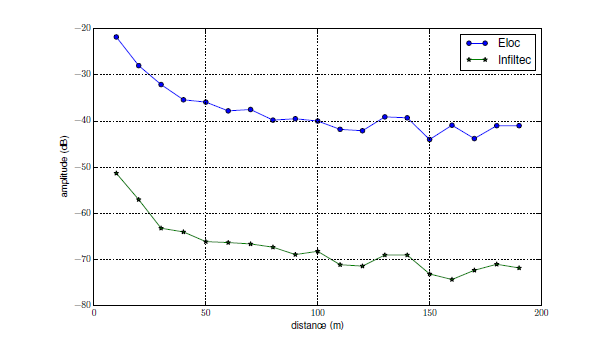
\includegraphics[width=10cm,height=13cm,keepaspectratio]{eloc_vs_infiltec2.png}
\caption[Sensitivity variation of the microphones with distance.]{Sensitivity variation of the microphones with distance.
The received power is measured for a 20 Hz tone
for different distances from a subwoofer. Eloc node outperforms
Infiltec device even for longer distances.}
\label{infiltec:eloc2}
\end{figure}

\subsection{Localization experiments}
\paragraph{}
Majority of the preliminary works were based on the correct localization of infrasound. Various experiments have been conducted at the University to achieve a better accuracy level of the localized angles using signal cross correlation technique. The method used for this experiment is explained in the methodology and design sections and only the result of these preliminary experiments are discussed in this section. The objectives of the following experiments are to calculate an angle of the direction of an infrasonic emitting sound source at different distances away from the source, estimate a formula for the error term, heuristically minimize the error by choosing a better sample rate and a statistical measure in calculating the angle. The distinction of these experiments is the use of a low-cost sensor made by us in the using off-the-shelf condenser microphones. This sensor  system consist of two microphones with a band pass filter.

\subsubsection{Localization experiment 01.}
\begin{figure}[H]
\centering
\begin{subfigure}{.5\textwidth}
  \centering
  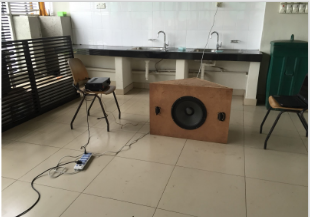
\includegraphics[width=.8\linewidth]{localizing_exp1_1.png}
  \caption{Infra sound emitting source}
  \label{fig:sub1}
\end{subfigure}%
\begin{subfigure}{.5\textwidth}
  \centering
  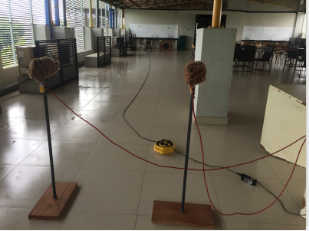
\includegraphics[width=.8\linewidth]{localizing_exp1_2.png}
  \caption{Elocate nodes placed 3m apart}
  \label{fig:sub2}
\end{subfigure}
\caption{Localizing experiment 01 setup}
\label{fig:test}
\end{figure}

\paragraph{}
The objective of this experiment was to calibrate the sensors and angle calculating program. This was done in indoors premises placing the speaker 10m away from the sensors and placing the two sensors 3m (Reasoning is in the chapter Design and Methodology ) apart from each other. Several recordings were taken by changing the angle between the imaginary line joining two sensors of a infrasonic tone played at 20hz frequency. The following table shows the result of this experiment. Left column of this table shows the actual or the real angle between the source and the hypothetical line joining two microphones, which has been calculated geometrically. The middle column show the estimated value of that angle and the right most column shows the difference between the actual and estimated angles.

\begin{table}[H]
\centering
\begin{tabular}{|m{0.3\textwidth}|m{0.3\textwidth}|m{0.2\textwidth}|} 
\hline
\bf {Actuale Angle} &  {\bf{ Estimated Angle }} & {\bf{ Difference }}\\
\hline
\hline
\bf {90} &  {\bf{ 88.6942 }} & {\bf{ 1.3058 }}\\
\hline
\bf {60} &  {\bf{ 67.2063 }} & {\bf{ 7.2063 }}\\
\hline
\bf {45} &  {\bf{ 43.7307 }} & {\bf{ 1.2693 }}\\
\hline
\bf {30} &  {\bf{ 38.0484 }} & {\bf{ 8.0484 }}\\
\hline
\bf {0} &  {\bf{ 17.4622 }} & {\bf{ 17.4622 }}\\
\hline
\end{tabular}
\end{table}

\subsubsection{Localization experiment 02.}

\paragraph{}
Following the correction of some errors in the angle calculating program and a modification of the gain in the sensors, the next experiment was conducted outdoors at the university grounds.  Similar to the indoor experiment, a low frequency was played from a specific position of the ground and recordings were taken from different places of the university.  Before estimating the angles, FFT was applied to the signals and the frequency against sample count was plotted, to check whether the played tone is received by the microphones. FFT graph of some of the audio clips are shown below. The frequency of the played wave during the experiment was 20Hz.


\paragraph{}
These angles were calculated by considering several windows from the recorded audio and the mode of the angles calculated in different windows were considered in this initial experiment.

\begin{figure}[H]
\centering

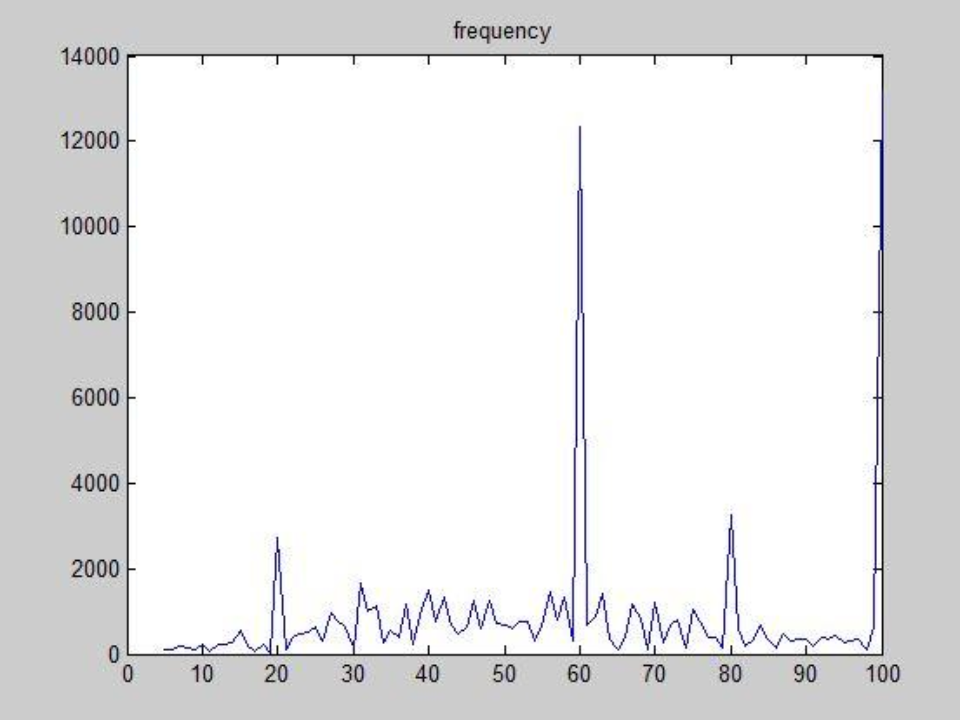
\includegraphics[width=10cm,height=13cm,keepaspectratio]{position3.png}
\caption{FFT at position 3}
\label{d:p3}
\end{figure}

\begin{figure}[H]
\centering
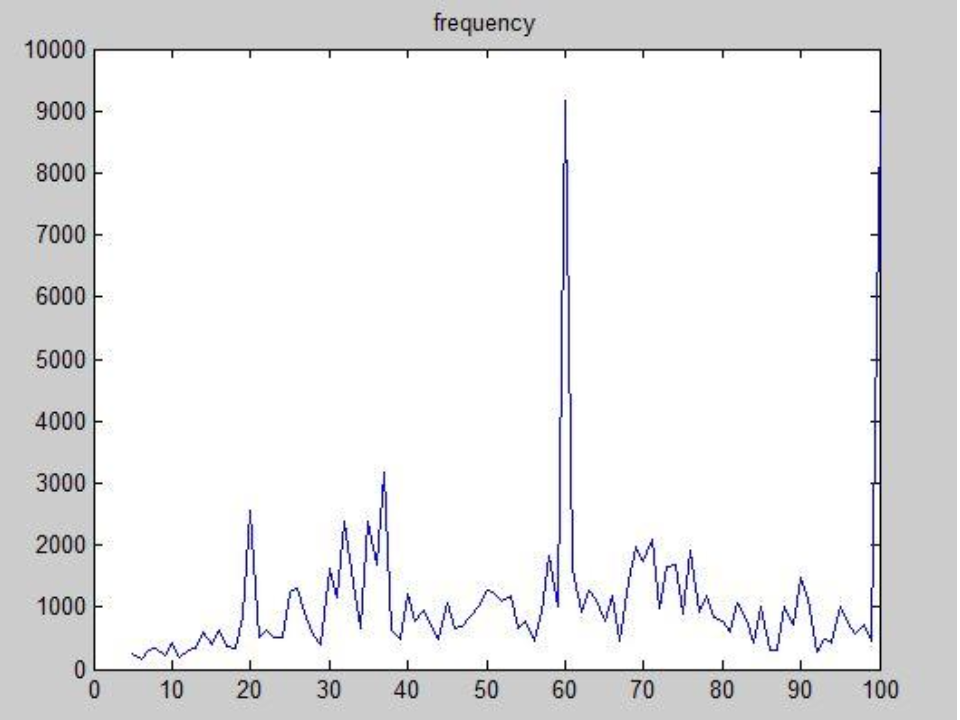
\includegraphics[width=10cm,height=13cm,keepaspectratio]{position7.png}
\caption{FFT at position 7}
\label{d:p7}
\end{figure}

\paragraph{}
Studying the above graphs, it is clear that the infrasonic waves reached two of the furthest recording places away from the speaker. Figure \ref{d:map} show the locations of the places where recordings were done.

\begin{figure}[H]
\centering
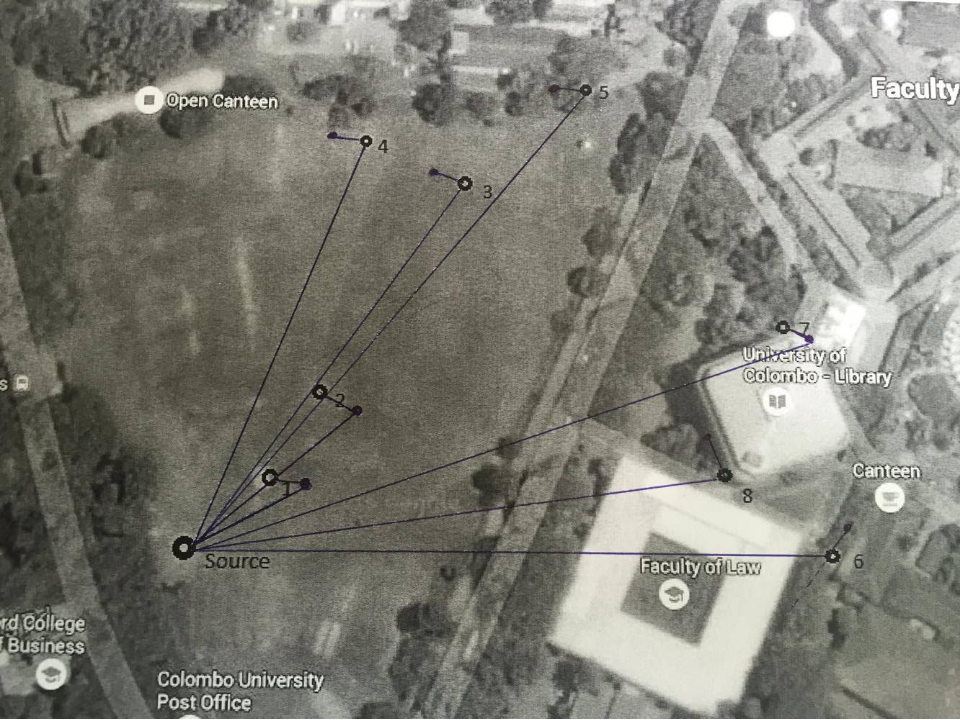
\includegraphics[width=14cm,height=11cm,keepaspectratio]{map.png}
\caption{Recording locations}
\label{d:map}
\end{figure}

\paragraph{}
The estimated angle and the actual angles of each positions can be found in the following table. Note that the actual angles are estimated geometrically using Google map.

\begin{table}[H]
\centering
\begin{tabular}{|m{0.3\textwidth}|m{0.3\textwidth}|m{0.2\textwidth}|} 
\hline
\bf {Actuale Angle} &  {\bf{ Calculated Angle }} & {\bf{ Difference }}\\
\hline
\hline
\bf {30} &  {\bf{ 25.209  }} & {\bf{ +4.791 }}\\
\hline
\bf {60} &  {\bf{ 59.574 }} & {\bf{ +0.426 }}\\
\hline
\bf {50} &  {\bf{ 48.457 }} & {\bf{ +1.543 }}\\
\hline
\bf {55} &  {\bf{ 59.909 }} & {\bf{ -4.909 }}\\
\hline
\bf {45} &  {\bf{ 45.153 }} & {\bf{ -0.153 }}\\
\hline
\bf {70} &  {\bf{ 65.692 }} & {\bf{ +4.308 }}\\
\hline
\bf {30} &  {\bf{ 26.912 }} & {\bf{ +3.088 }}\\
\hline
\end{tabular}
\end{table}

\newpage
\subsubsection{Localization experiment 03.}
\paragraph{}
In this experiment place a pair of Eloc nodes in an open field and place the subwoofer in different locations around the node pair to get different angles. We maintain a constant distance of 20 meters between the subwoofer and the Eloc node pair in each of our placements. The distance between the two Eloc nodes has an effect on the capability to localize low frequency sounds using the method explained previously. The rationale of selecting this distance is as follows:

\paragraph{}
The angle calculation equation compares two signals using cross correlation and finds the phase difference between
them in terms of sample lags. If two signals coming from the node pair are in a 180\textsuperscript{o} degrees or a higher phase difference,the correlation and sample lag calculation phase may incorrectly detect it as a different phase. To avoid such scenarios,the distance between two Eloc nodes should be equal to or less than the wavelength of the frequency we use for the localization. We therefore select 3 meters as the distance between the Eloc nodes which is roughly the wavelength of the frequency 120 Hz under the atmospheric temperature of 30\textsuperscript{o} C. This selection enables us to use frequencies below 120 Hz for the localization which includes a number of higher harmonics in addition to the fundamental frequency components of the elephants in the infrasonic range. The speed of sound v in dry air when the temperature is T Celsius is given by the following formula.

\begin{equation}
v = 331.4+0.6T m/s
\end{equation}
\paragraph{}
At the time of this experiments, the temperature of the atmosphere at the location was approximately
30\textsuperscript{o} C and therefore the speed of sound was considered as 350 ms\textsuperscript{-1} in the calculations. The sampling rate of the Eloc nodes is set to 44100 Hz.
\paragraph{}
In this experiment, instead of taking out the mod value of the angles calculated in different windows, a histogram was plotted for the angle distribution. As in the above experiment, the sound source was placed at the same location and recordings were taken at different angles between the source and the sensors. This time, actual angles were calculated geometrically at the location using basic simple geometric construction theories. The following table shows the results related to the experiment. 'x' axis will indicate the angle from 0 to 90 in degrees and 'y' axis will indicate the number of windows which estimated within each range.  


\begin{figure}[H]
  \centering
  \begin{minipage}[b]{0.4\textwidth}
    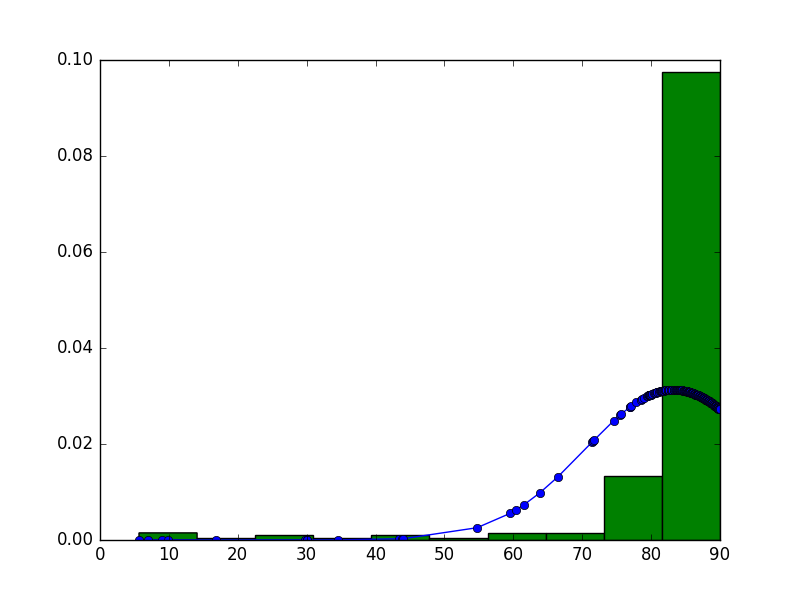
\includegraphics[width=\textwidth]{angle90.png}
    \caption[Estimation at angle 90 degrees]{90 degrees.
	\\\hspace{\textwidth}Mode   = 89.70983873 , count=28
	\\\hspace{\textwidth}	Median=86.5159328561
	\\\hspace{\textwidth}	Mean   =83.2375912981
	\\\hspace{\textwidth}	SD       =12.7332313597   
    }
  \end{minipage}
  \hfill
  \begin{minipage}[b]{0.4\textwidth}
    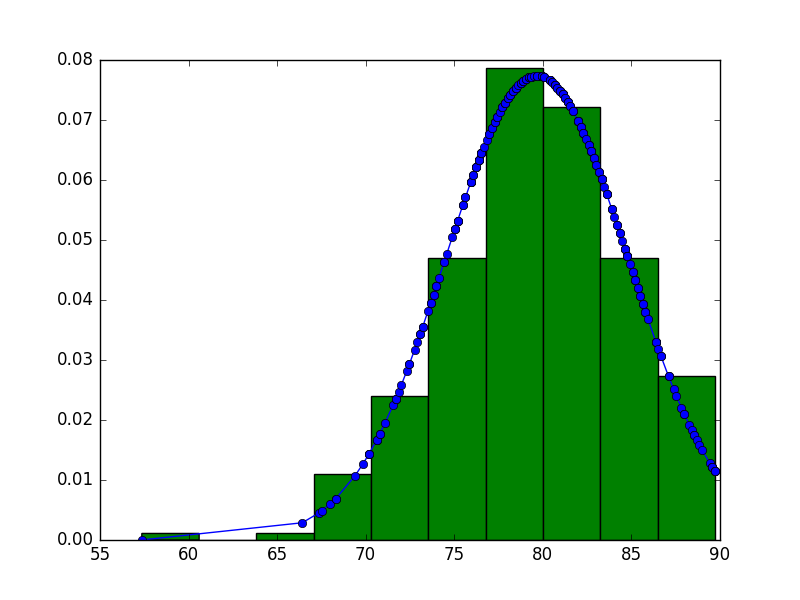
\includegraphics[width=\textwidth]{angle80.png}
    \caption[Estimation at angle 80 degrees]{80 degrees.
    \\\hspace{\textwidth}Mode   = 81.99457761, count=8
	\\\hspace{\textwidth}	Median=79.6430076398
	\\\hspace{\textwidth}	Mean   =79.6490254668
	\\\hspace{\textwidth}	SD       =5.15568710347 }
  \end{minipage}
\end{figure}


\begin{figure}[H]
  \centering
  \begin{minipage}[b]{0.4\textwidth}
    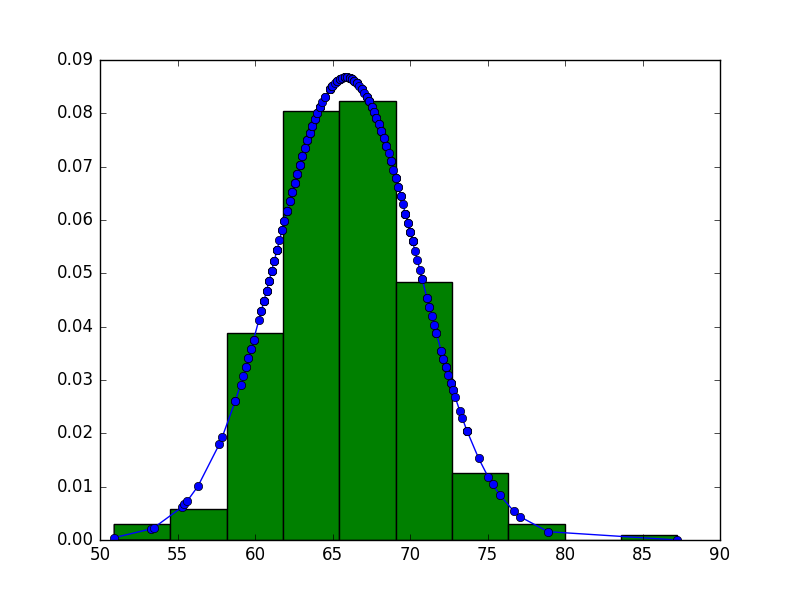
\includegraphics[width=\textwidth]{angle70.png}
    \caption[Estimation at angle 70 degrees]{70 degrees.
    \\\hspace{\textwidth}Mode   = 64.82421625, count=8
	\\\hspace{\textwidth}	Median=65.8618349913
	\\\hspace{\textwidth}	Mean   =65.8607911578
	\\\hspace{\textwidth}	SD       =4.59936937079}
  \end{minipage}
  \hfill
  \begin{minipage}[b]{0.4\textwidth}
    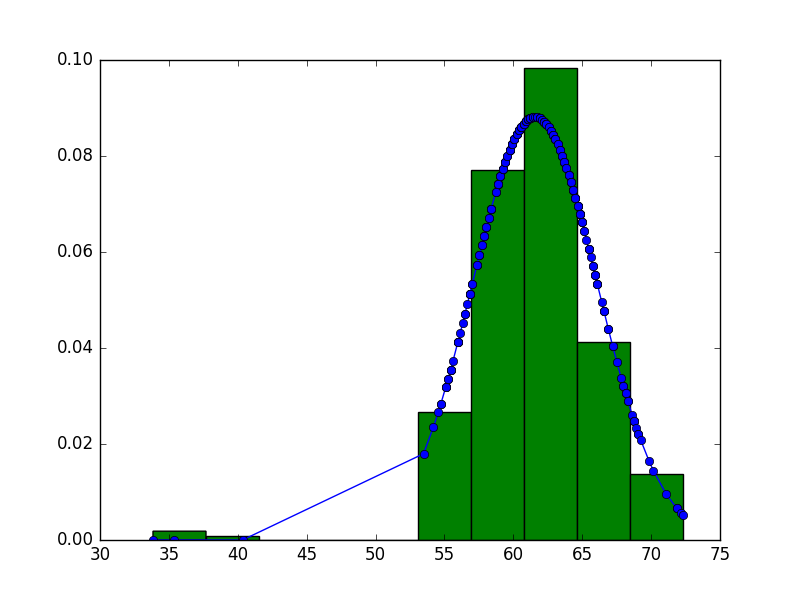
\includegraphics[width=\textwidth]{angle60.png}
    \caption[Estimation at angle 60 degrees]{60 degrees.
     \\\hspace{\textwidth}Mode   = 60.91098812, count=8
	\\\hspace{\textwidth}	Median=61.4078587362
	\\\hspace{\textwidth}	Mean   =61.5563084786
	\\\hspace{\textwidth}	SD       =4.52718225527}
  \end{minipage}
\end{figure}
\begin{figure}[H]
  \centering
  \begin{minipage}[b]{0.4\textwidth}
    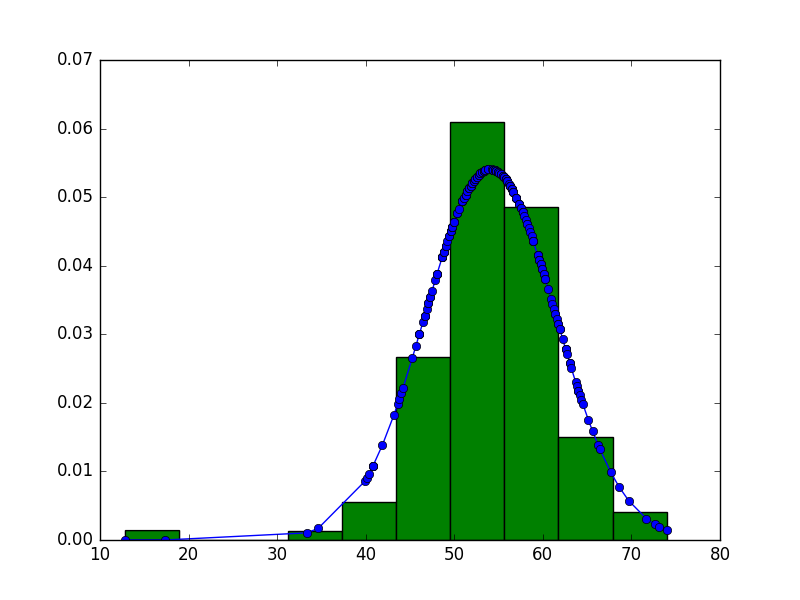
\includegraphics[width=\textwidth]{angle50.png}
    \caption[Estimation at angle 50 degrees]{50 degrees.
    \\\hspace{\textwidth}Mode   = 48.63264645, count=6
	\\\hspace{\textwidth}	Median=54.3812862719
	\\\hspace{\textwidth}	Mean   =54.0619896404
	\\\hspace{\textwidth}	SD       =7.37749397882}
  \end{minipage}
  \hfill
  \begin{minipage}[b]{0.4\textwidth}
    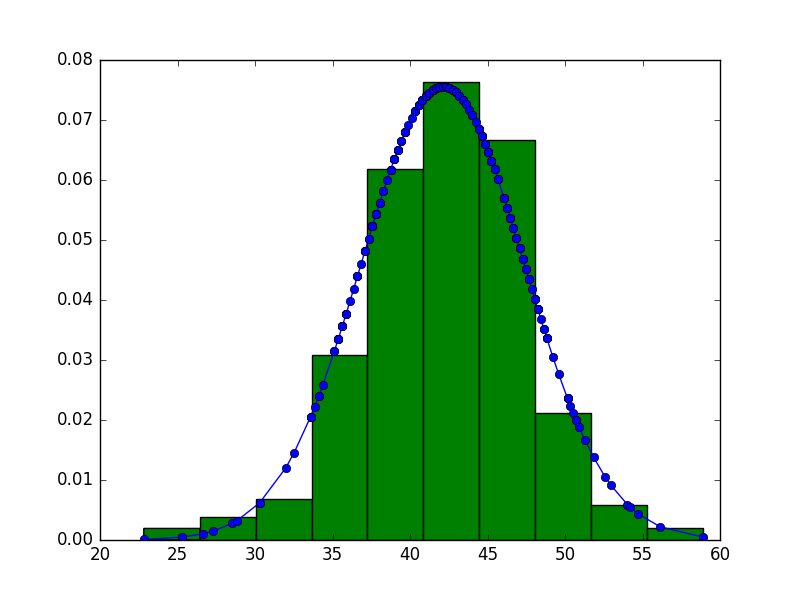
\includegraphics[width=\textwidth]{angle40.png}
    \caption[Estimation at angle 40 degrees]{40 degrees.
    \\\hspace{\textwidth}Mode   = 37.57509342, count=11
	\\\hspace{\textwidth}	Median= 41.888596915
	\\\hspace{\textwidth}	Mean   = 42.1067250378
	\\\hspace{\textwidth}	SD       = 5.27880107871}
  \end{minipage}
\end{figure} 
\begin{figure}[H]
  \centering
  \begin{minipage}[b]{0.4\textwidth}
    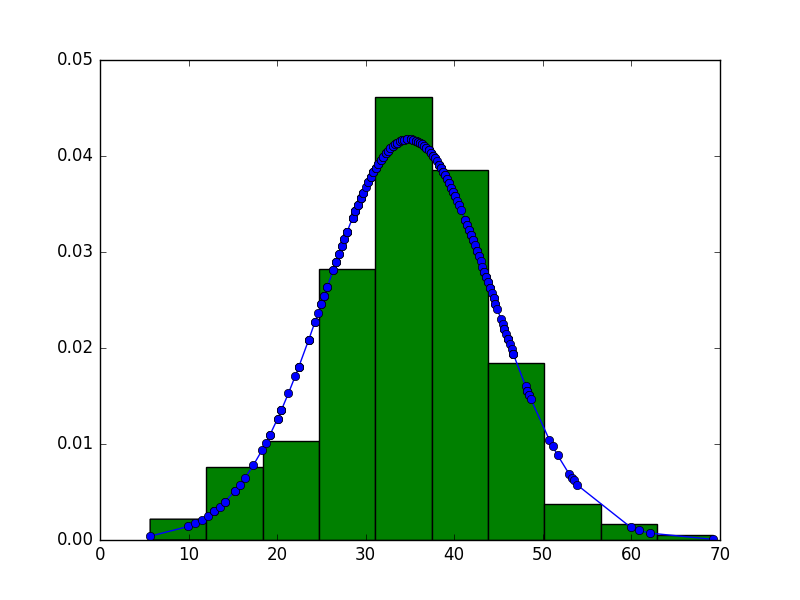
\includegraphics[width=\textwidth]{angle30.png}
    \caption[Estimation at angle 30 degrees]{30 degrees.
    \\\hspace{\textwidth}Mode   = 33.58472103, count=7
	\\\hspace{\textwidth}	Median= 35.5035252434
	\\\hspace{\textwidth}	Mean   = 34.8220985845
	\\\hspace{\textwidth}	SD       = 9.55595652093}
  \end{minipage} 
  \hfill
  \begin{minipage}[b]{0.4\textwidth}
    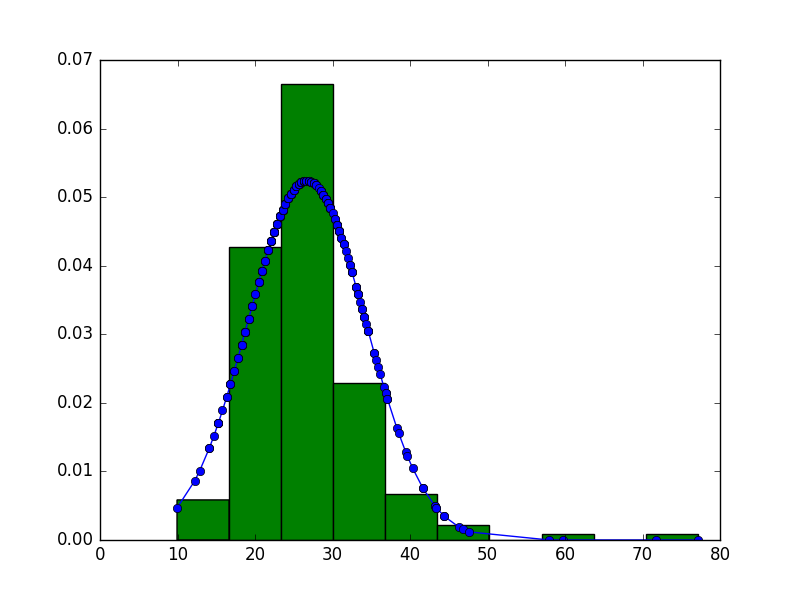
\includegraphics[width=\textwidth]{angle20.png}
    \caption[Estimation at angle 20 degrees]{20 degrees
    \\\hspace{\textwidth}Mode   = 28.52041819, count=16
	\\\hspace{\textwidth}	Median= 27.9066563489
	\\\hspace{\textwidth}	Mean   = 27.495790336
	\\\hspace{\textwidth}	SD       = 5.63783305083}
  \end{minipage}
\end{figure}
\begin{figure}[H]
  \centering
  \begin{minipage}[b]{0.4\textwidth}
    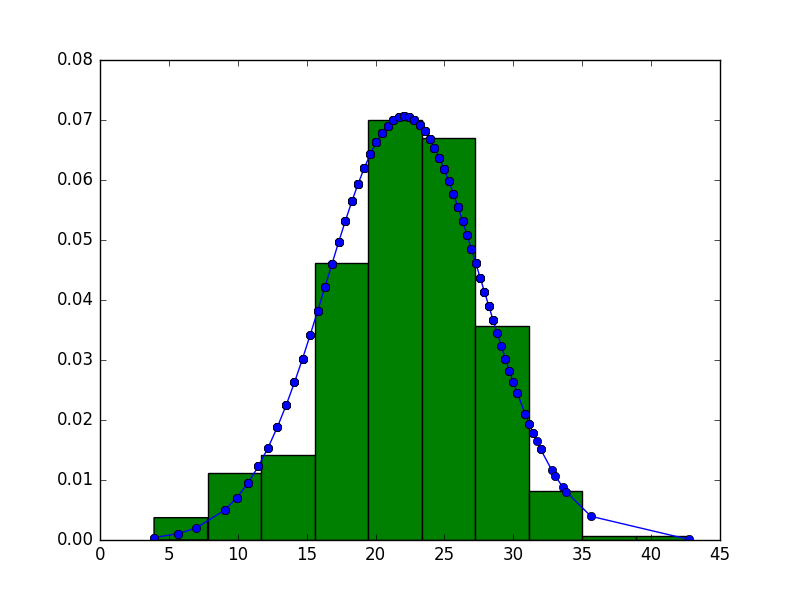
\includegraphics[width=\textwidth]{angle10.png}
    \caption[Estimation at angle 10 degrees]{10 degrees.
    \\\hspace{\textwidth}Mode   = 20.04595607, count=13
	\\\hspace{\textwidth}	Median= 22.8251265163
	\\\hspace{\textwidth}	Mean   = 22.0617301801
	\\\hspace{\textwidth}	SD       = 5.65022211431}
  \end{minipage}
  \hfill
  \begin{minipage}[b]{0.4\textwidth}
    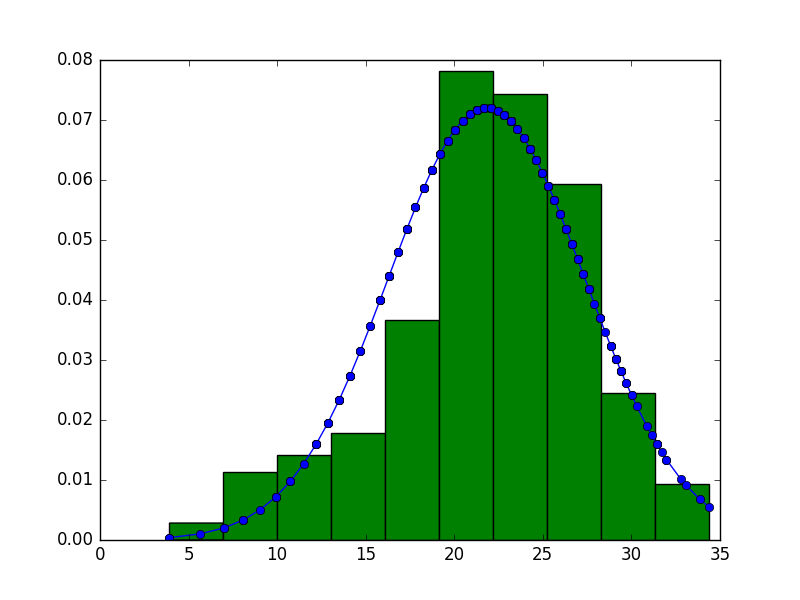
\includegraphics[width=\textwidth]{angle0.png}
    \caption[Estimation at angle 0 degrees]{0 degrees.
    \\\hspace{\textwidth}Mode   = 23.19626789, count=17
	\\\hspace{\textwidth}	Median= 22.4481828776
	\\\hspace{\textwidth}	Mean   = 21.8176255333
	\\\hspace{\textwidth}	SD       = 5.54044788287}
  \end{minipage}
\end{figure}
\paragraph{}
The following table shows the number of windows, which has been produced in the correct range as well as the total number of windows.

\begin{table}[H]
\centering
\begin{tabular}{|m{0.2\textwidth}|m{0.2\textwidth}|m{0.2\textwidth}|m{0.2\textwidth}|} 
\hline
\bf {Actuale Angle} &  {\bf{ Estimated Range }} & {\bf{ Window count }} & {\bf{Total window count}}\\
\hline
\hline
\bf {0} &  {\bf{ 0-7.2  }} & {\bf{250 }} & {\bf{ 402 }}\\
\hline
\bf {10} &  {\bf{ 7.9-11.6 }} & {\bf{85 }} & {\bf{ 345 }}\\
\hline
\bf {20} &  {\bf{ 24.7-27.4 }} & {\bf{65 }} & {\bf{ 347 }}\\
\hline
\bf {30} &  {\bf{ 26.4-30.8 }} & {\bf{120 }} & {\bf{ 331 }}\\
\hline
\bf {40} &  {\bf{ 30.8-34.9 }} & {\bf{120 }} & {\bf{ 310 }}\\
\hline
\bf {50} &  {\bf{ 34-41.5 }} & {\bf{100 }} & {\bf{ 332 }}\\
\hline
\bf {60} &  {\bf{ 46-50}} & {\bf{ 110}} & {\bf{ 460 }}\\
\hline
\bf {70} &  {\bf{ 53-62 }} & {\bf{ 55 }} & {\bf{ 366}}\\
\hline
\bf {80} &  {\bf{ 65-69 }} & {\bf{ 110 }} & {\bf{ 431 }}\\
\hline
\bf {90} &  {\bf{ 65-79 }} & {\bf{ 110 }} & {\bf{ 384}}\\
\hline
\bf {90} &  {\bf{ 70-73 }} & {\bf{ 90 }} & {\bf{ 507}}\\
\hline
\end{tabular}
\end{table}

\paragraph{}
For the considered angle range
from 0\textsuperscript{o} to 90\textsuperscript{o} degrees, there is an error in the calculated angle which makes it different from the real angle. This error is illustrated in Figure 10 b. The figure \ref{error:angle} (b) shows that the calculated error is large for the angles closer to 0\textsuperscript{o} and gets smaller as the angles get close to 90\textsuperscript{o}which corresponds to the theoretical foundation laid in the chapter 2. For an angle of 0\textsuperscript{o} degrees, the theoretical value we get should be infinite. However, due to the measurement and random errors in experiments, the angle is not infinite but as high as 17\textsuperscript{o}. For all the other angles approaching 90\textsuperscript{o} degrees the error is quite low as Figure  \ref{error:angle} (b) shows. For the range between 30\textsuperscript{o} to 90\textsuperscript{o} angles, we get an average error which is approximately 1.8\textsuperscript{o} and a maximum error of 4.5\textsuperscript{o}. This result indicates that we can reliably use an angle value calculated using a pair of Eloc nodes if the angle to the infrasonic source is greater than approximately 30\textsuperscript{o} degrees. By using multiple pairs of Eloc nodes deployed at different angles to each other, we can select the most reliable node pairs for the final location by ignoring the ones which measure an angle less than 30\textsuperscript{o} degrees to the infrasonic source. 
\begin{figure}[H]
\centering
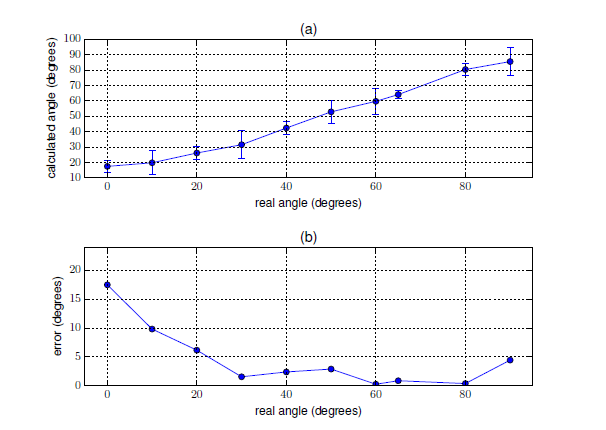
\includegraphics[width=10cm,height=13cm,keepaspectratio]{error_angles.png}
\caption[Accuracy of calculating the direction to an infrasonic
source using a pair of Eloc nodes.]{Accuracy of calculating the direction to an infrasonic
source using a pair of Eloc nodes. The top part of the Figure shows the relationship between real angles and respective
calculated angles. The lower part shows the variation of
the error in calculation against the real angle in consideration.
For angles above 30 degrees the error is low.}
\label{error:angle}
\end{figure}

\subsection{Elephant Sound Recording in the Wild}

\paragraph{}
The previous experiments confirm that Eloc nodes together with the wind shield can identify infrasonic frequencies inside the controlled environment of a laboratory even when there is wind. However, real deployments pose further challenges such as vehicle noise from nearby areas, vibrations that occur on the Eloc nodes due to the impact of dust and vegetation in the deployed location. Therefore, we evaluate the effectiveness of Eloc nodes to identify low frequency elephant sounds in the wild. In order to capture real elephant sounds, we take a pair of Eloc nodes to a national park in Sri Lanka where elephants roam freely.
\subsubsection{At Kalawewa Sanctuary }
\paragraph{}
First, the recording was done in a national park situated in Anuradhapura district bounded to the Kalawewa tank. We placed our Elocate nodes in a bathing area of elephants and initiated recording once the arrival of an elephant was detected. Recordings were done for about 5 hours per day and this was performed for two days. All the observations and hearings were noted down for future annotation of the data. Following are some photographs taken during this period. 
 
\begin{figure}[H]
\centering
\begin{subfigure}{.5\textwidth}
  \centering
  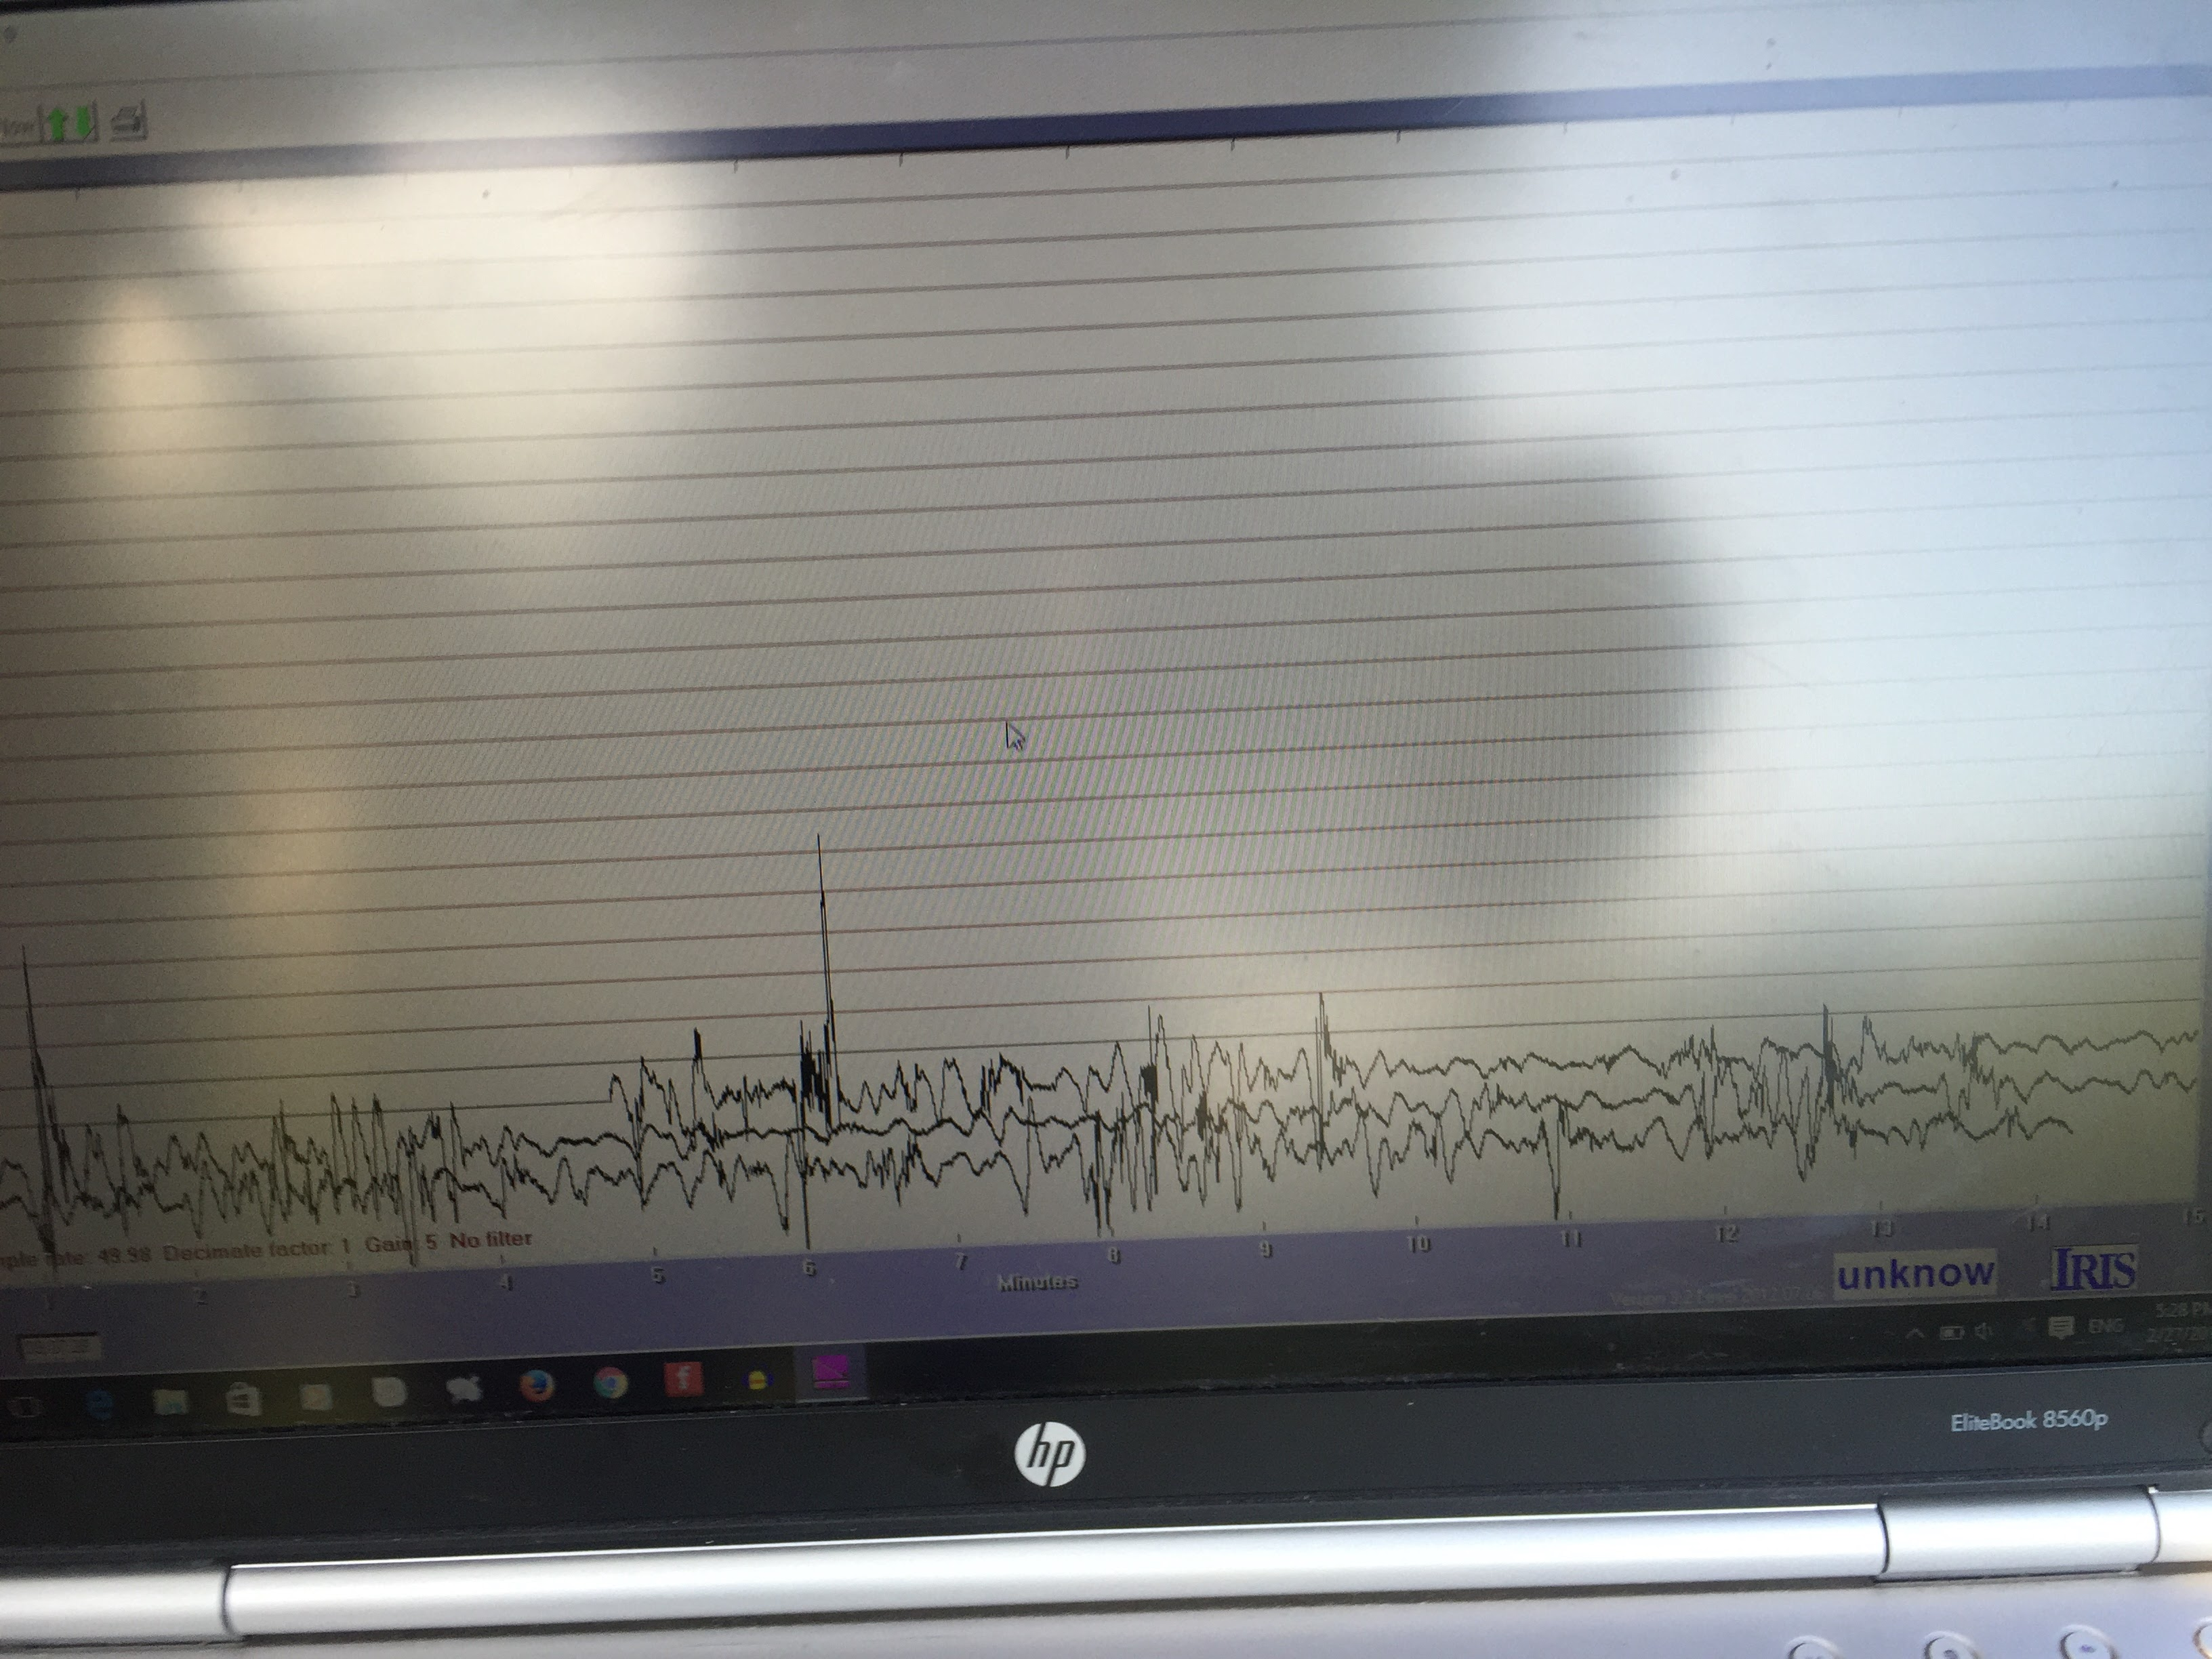
\includegraphics[width=.8\linewidth]{Kalawewa1.jpg}
  \caption{Waveform of the audio.}
  \label{fig:sub1}
\end{subfigure}%
\begin{subfigure}{.5\textwidth}
  \centering
  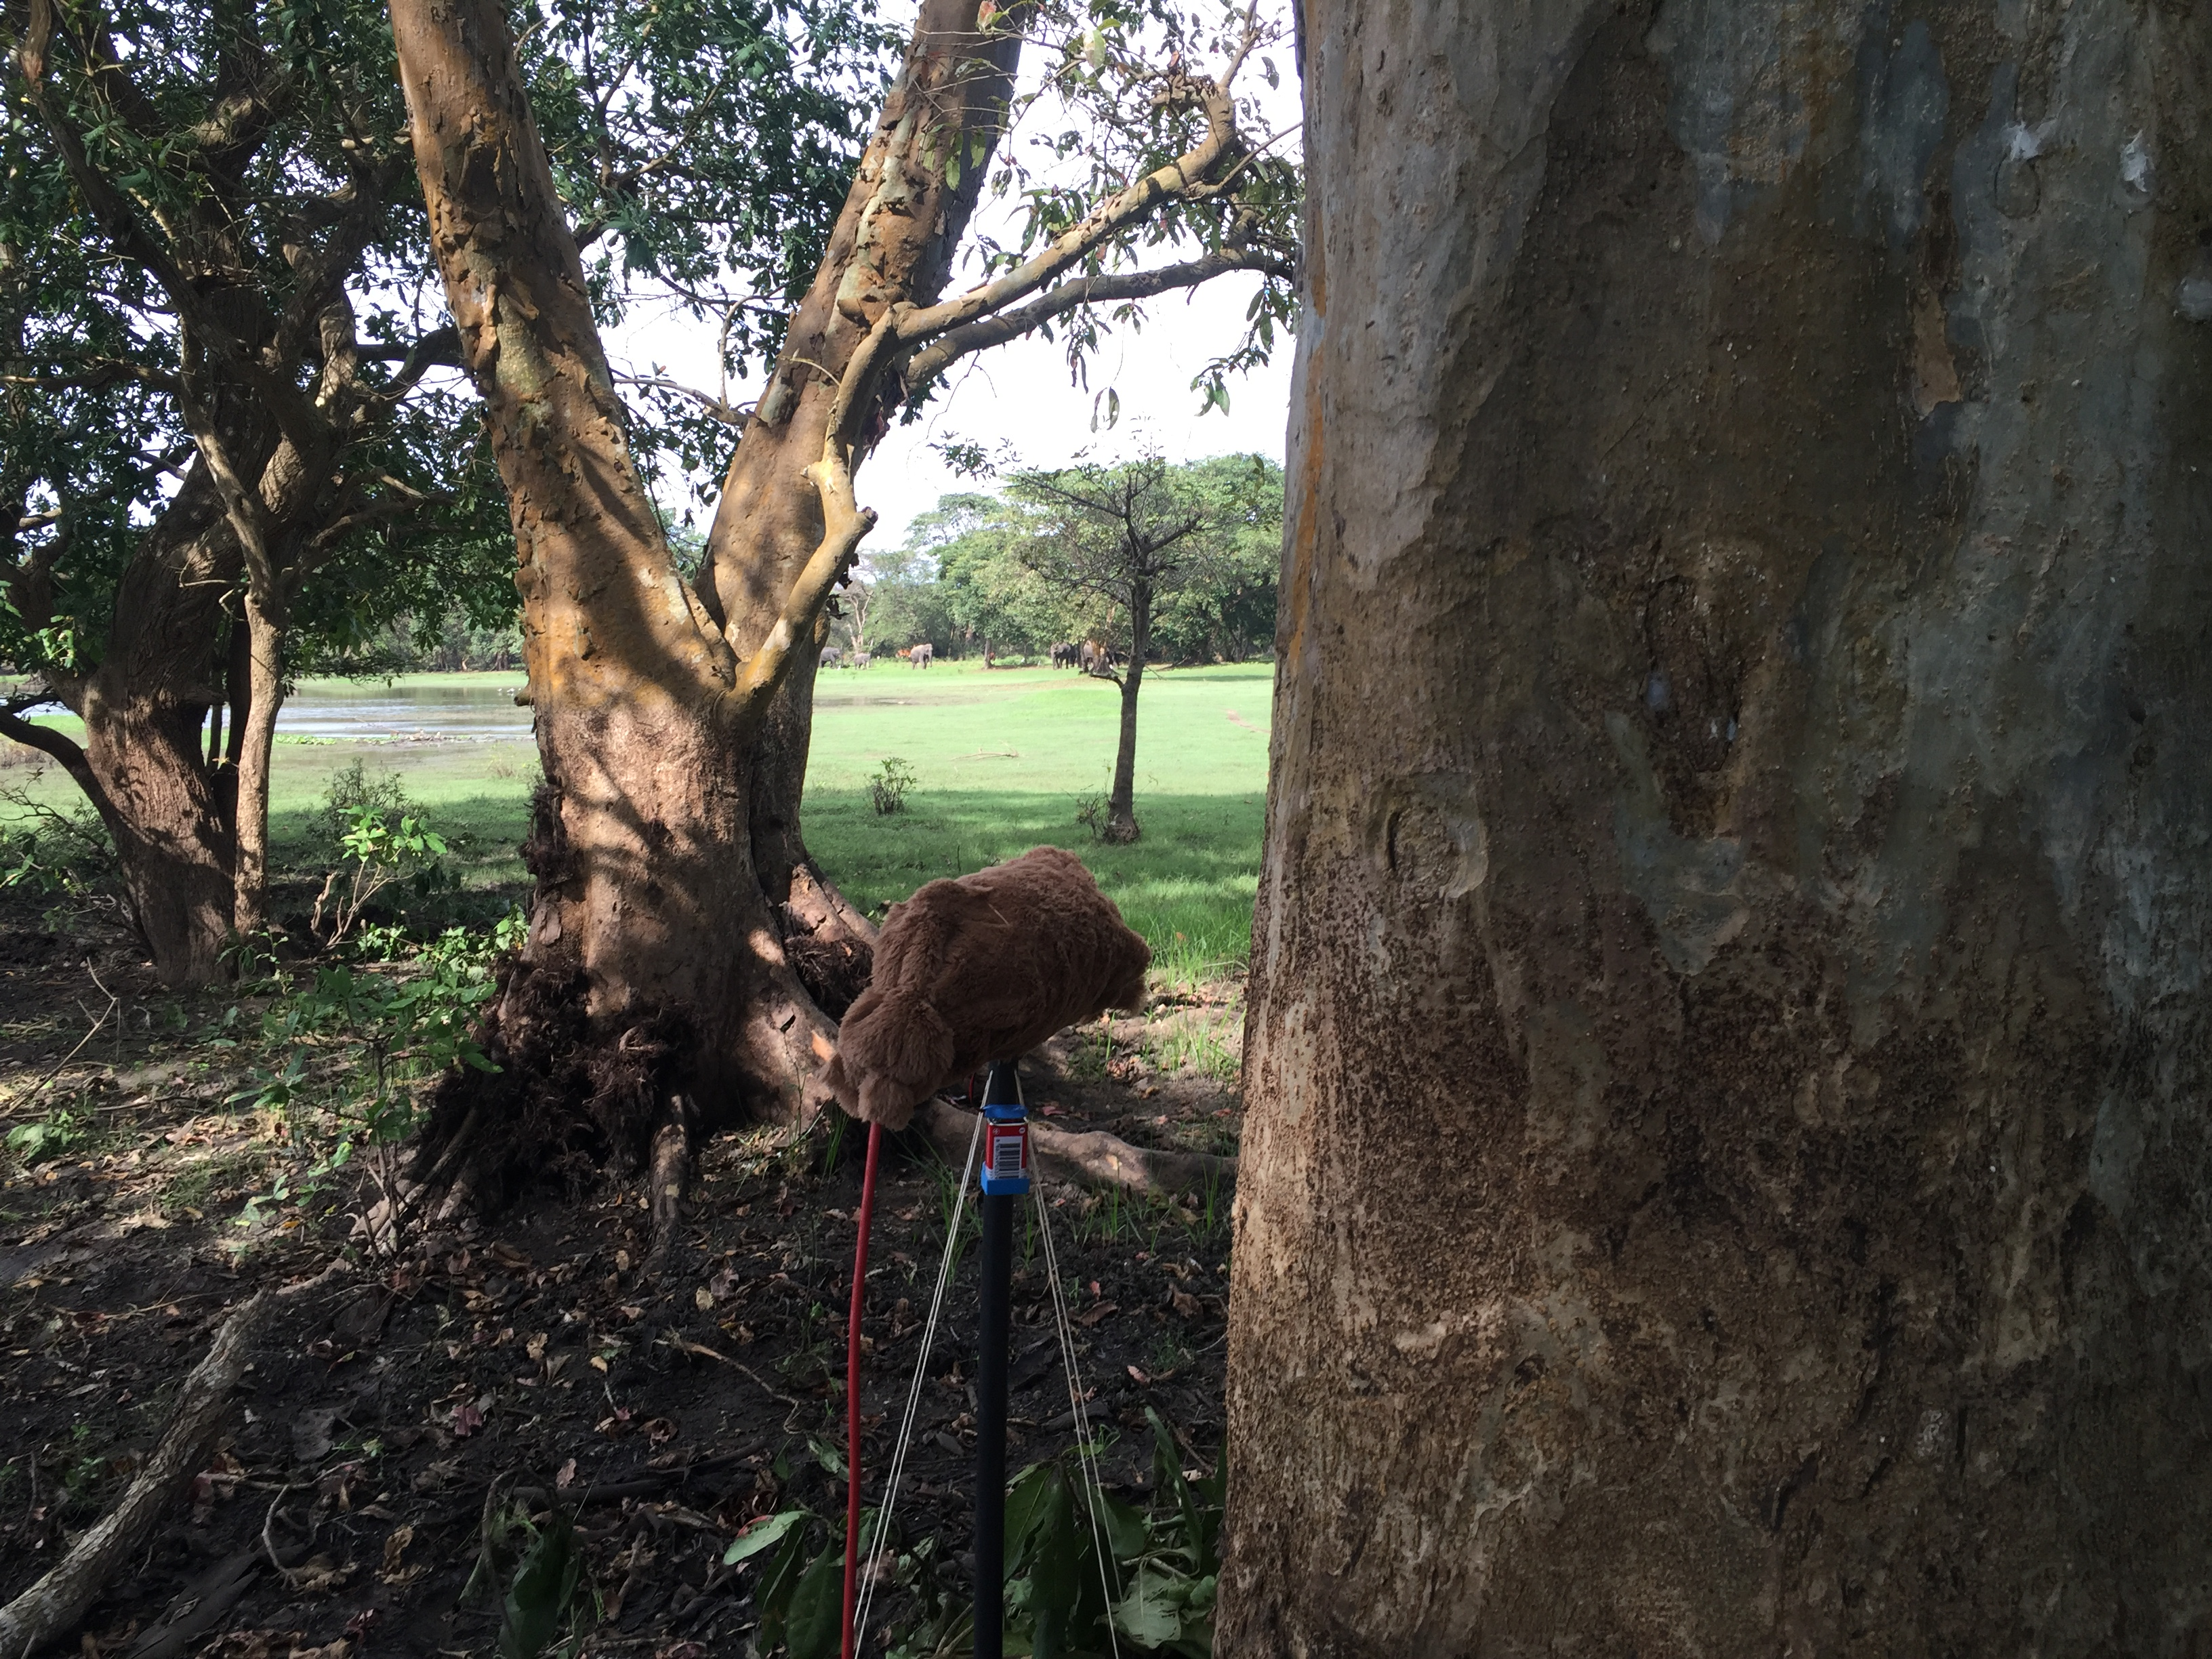
\includegraphics[width=.8\linewidth]{Kalawewa2.jpg}
  \caption{An Elocate node placed in the wild}
  \label{fig:sub2}
\end{subfigure}
\caption{Images of the devices while recording}
\label{fig:test}
\end{figure} 

\begin{figure}[H]
\centering
\begin{subfigure}{.5\textwidth}
  \centering
  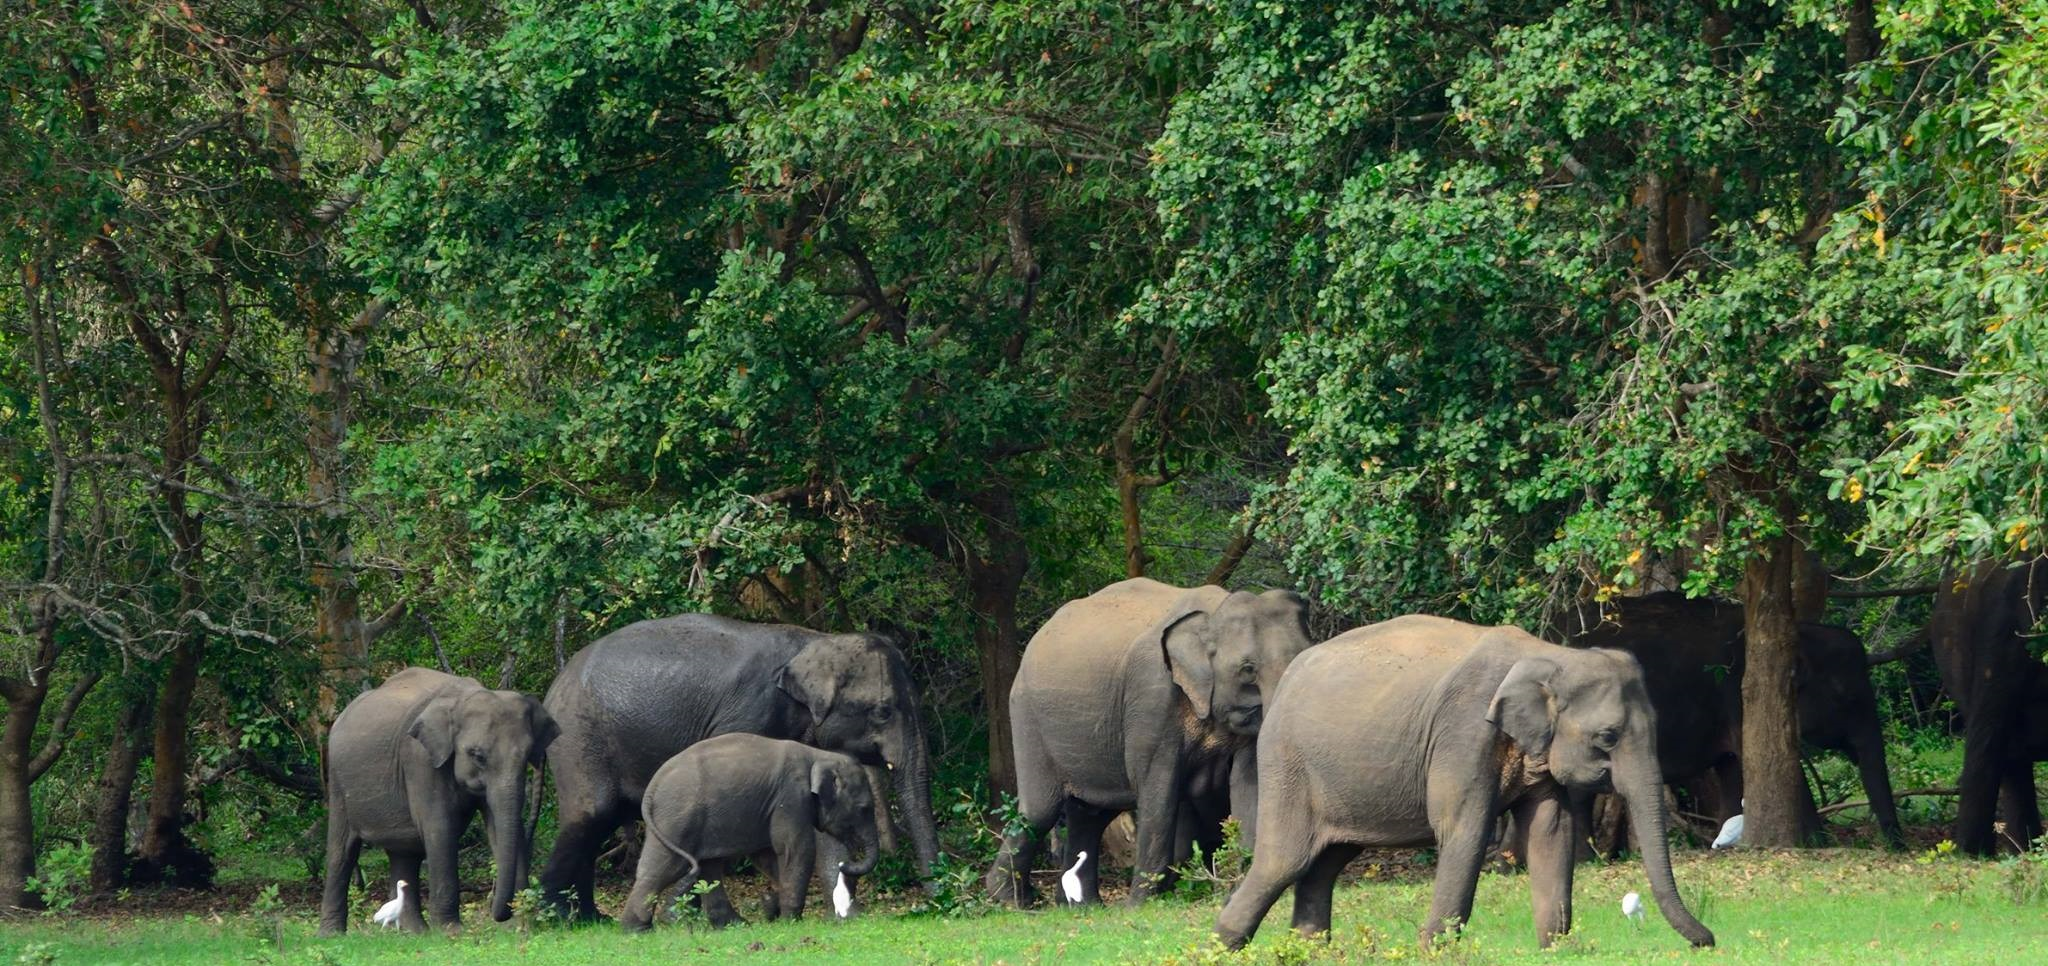
\includegraphics[width=.8\linewidth]{Kalawewa4.jpg}
  \caption{An elephant heard entering to the tank.}
  \label{fig:sub1}
\end{subfigure}%
\begin{subfigure}{.5\textwidth}
  \centering
  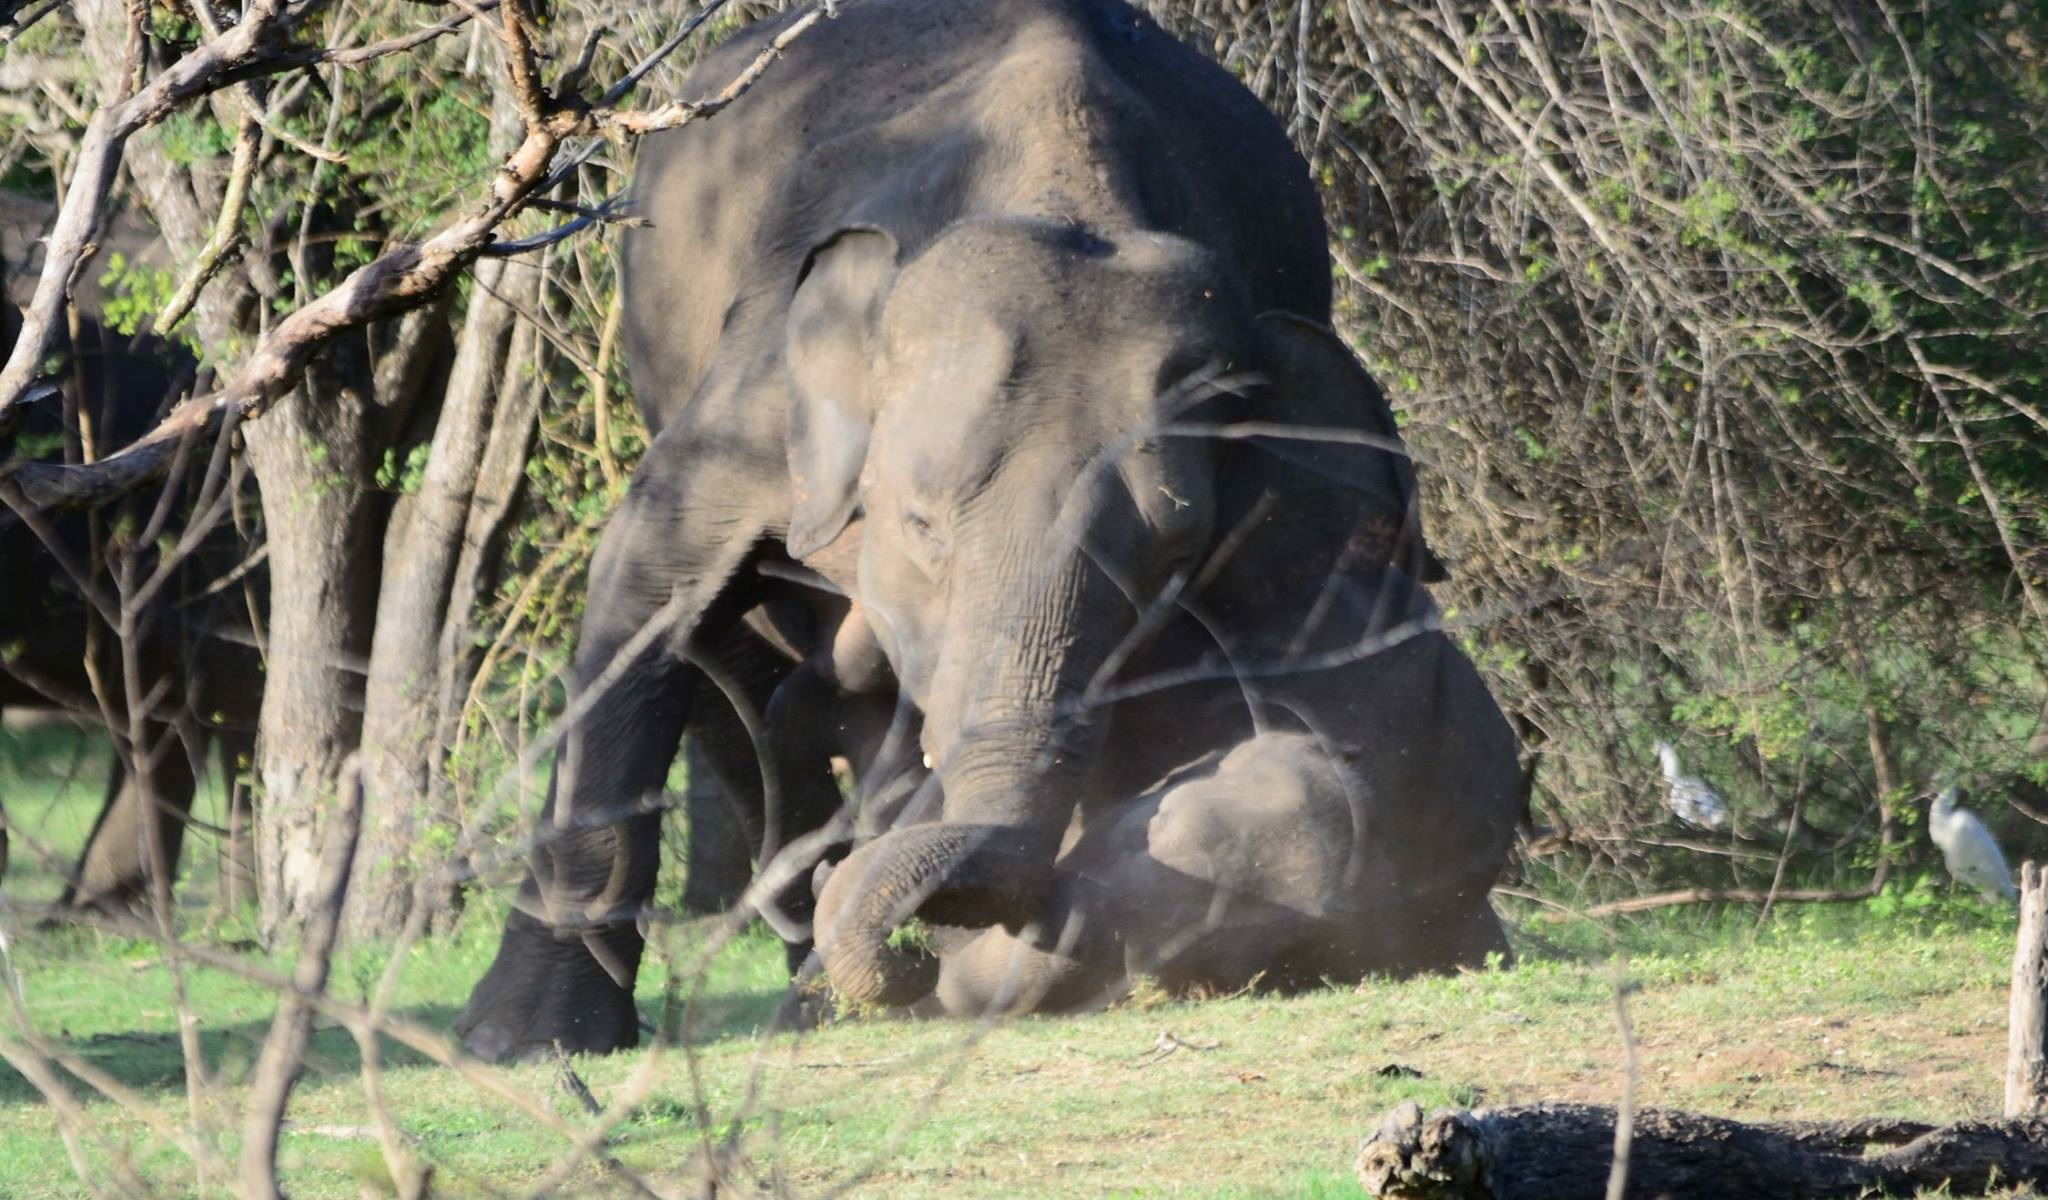
\includegraphics[width=.8\linewidth]{Kalawewa5.jpg}
  \caption{A female elephant attacking to a young male elephant}
  \label{fig:sub2}
\end{subfigure}
\caption{Images of the activities done by elephants}
\label{fig:test}
\end{figure} 
 
 
\subsubsection{At Yala National Park} 
\paragraph{}
We mounted the nodes inside an off road vehicle and parked it in a location inside the national park where it is possible to observe elephants visually while recording sounds. The vehicle engine was turned off during the time of recording. Other external noise sources such as wind and vehicles in the nearby areas were present. We noted the presence of elephants and their behavior in the visual range and compared them against the data recorded. We obtained the support of a zoologist to verify whether the recorded patterns are from an elephant.
\paragraph{}
Figure \ref{waveform:specto} illustrates the waveform, frequency domain and the spectrogram of an elephant sound identified by
a zoologist from our field recordings. As the figure shows, Eloc nodes can clearly capture the fundamental frequency
component of the sound that is below the 25 Hz in addition to the higher frequency harmonics. However, due to the effect
of the low-pass filter in Eloc nodes, the frequencies above 150 Hz are significantly attenuated.

\begin{figure}[H]
\centering
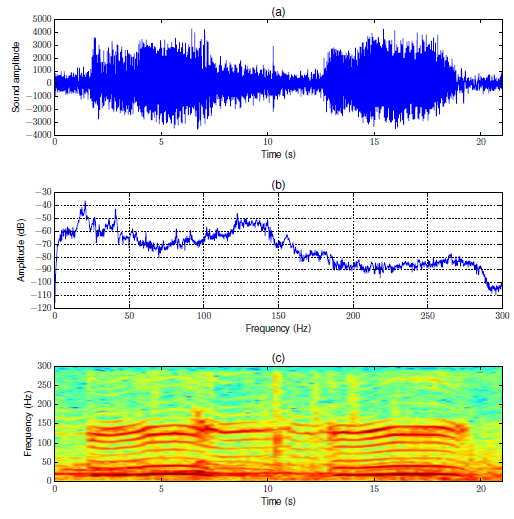
\includegraphics[width=10cm,height=13cm,keepaspectratio]{wild_recordings.png}
\caption[Waveform and spectrogram of a recording]{An excerpt from the elephant sound recordings using
a pair of Eloc nodes. The graph (a) shows the waveform
of the signal while the graph (b) shows its frequency domain.
Graph (c) illustrates the spectrogram of the signal where a
number of higher harmonics of the fundamental frequency of
the elephant sound is visible. (The waveform shown in graph
(a) has the amplitude as a scalar value between +215 and
+215 since we store the recorded data in wave files which
uses 16-bit Pulse Code Modulation (PCM))}
\label{waveform:specto}
\end{figure}


\paragraph{}
During the visit to Yala, we were able to  record data that could also be used for the purpose of localization. We perform most of the evaluations using an artificial infrasonic source due to the inability to conduct repeatable experiments using a real elephant in the wild. Even though it is hard to verify the results of a localization experiments we perform in the wild, such trials are necessary to build the confidence that Eloc works in real scenarios. During a one such scenario we were able to observe a moving heard of elephants making loud rumbles. While recording elephant sounds with the microphones, we visually observed the elephants and their movements and continuously calculated the angle to their position.

\begin{figure}[H]
\centering
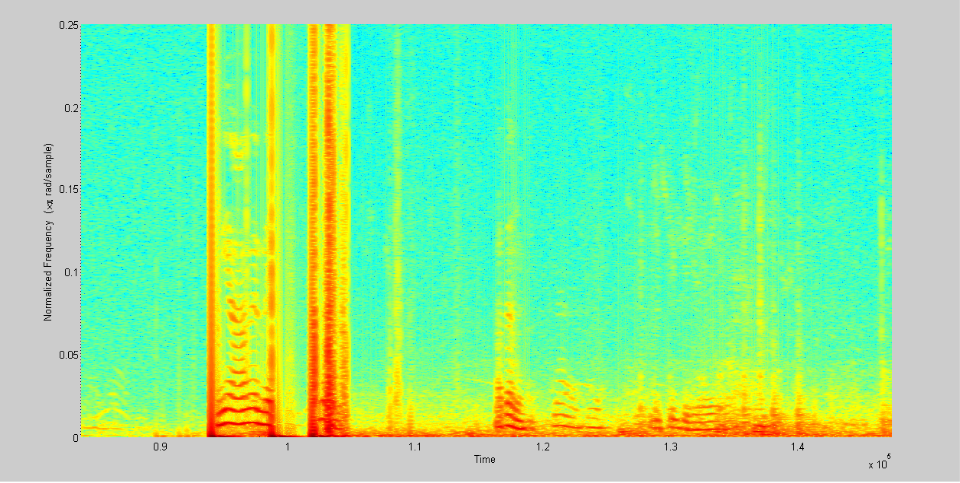
\includegraphics[width=14cm,height=11cm,keepaspectratio]{44100.png}
\caption{Spectogram of the signal under 44100 sample rate}
\label{d:44100}
\end{figure}

The above image shows the spectrogram of a recorded clip at a sample rate of 44100 . The patterns of elephant rumbles are shown by the small red curves \cite {19}. If the above clip re-sampled at sample rate of 250 , the infrasonic rumble patterns become visible.

\begin{figure}[H]
\centering
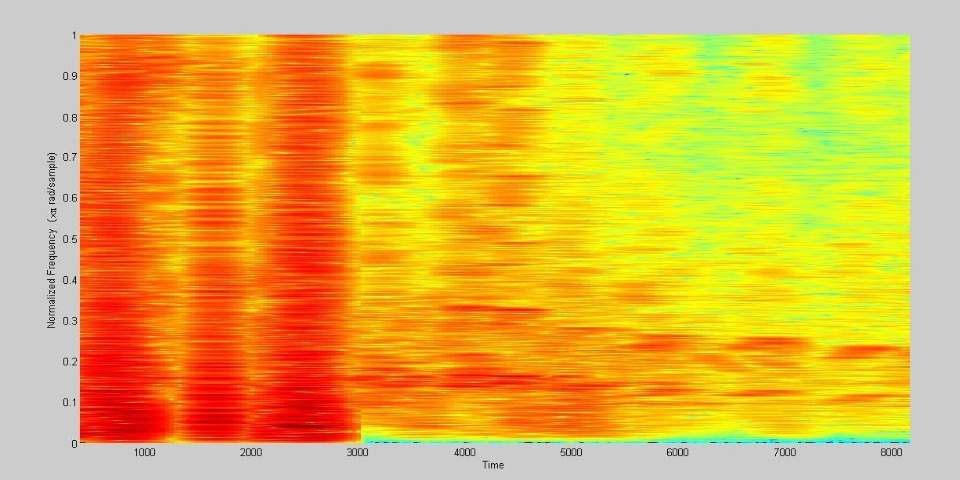
\includegraphics[width=14cm,height=11cm,keepaspectratio]{200.png}
\caption{Spectogram of the signal under 200 sample rate}
\label{d:200}
\end{figure}

\paragraph{}
Figure \ref{yalascene} illustrates a localization scenario we came across in such a field experiment. We observed an elephant moving from an open area into the jungle where the thick vegetation blocked the visibility of the elephant from
the location of the vehicle. From the infrasonic signal patterns we captured during the elephants movement, we calculated
the angle to the elephant at different time intervals. The values of the calculated angles are X1 = 47.5\textsuperscript{o}, X2 = 41.5\textsuperscript{o}, X3 = 35\textsuperscript{o}, X4 = 34\textsuperscript{o} and X5 = 32.5\textsuperscript{o}. As Figure \ref{yalascene} illustrates, the angles we compute agree with the elephants movement direction we observed visually.
And an estimation of the angle ranges in each continuous clip is given in the table below.

\begin{figure}[H]
\centering
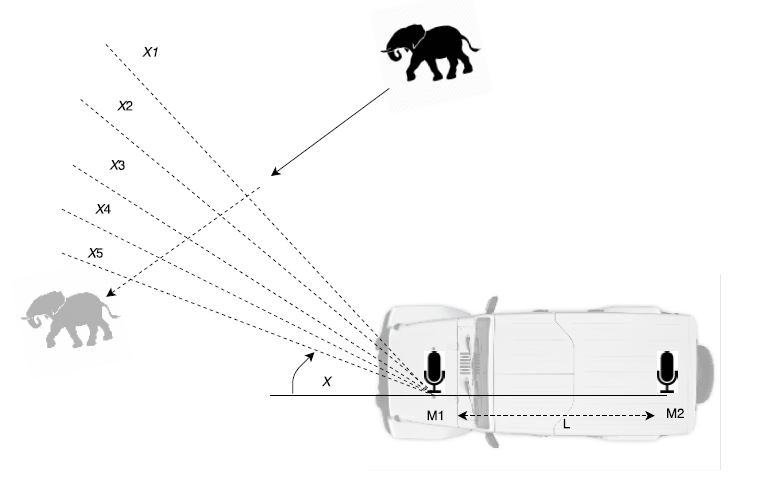
\includegraphics[width=14cm,height=11cm,keepaspectratio]{yalascene.png}
\caption[A recording scenario at Yala]{We mounted two Eloc nodes in the front and back
of a jeep and calculated the angles of infrasonic emissions received
from a moving elephant from a visible location into
the thick jungle. The values of the calculated angles agree
with the visual observation of the elephants movement direction.}
\label{yalascene}
\end{figure}


\begin{table}[H]
\centering
\begin{tabular}{|m{0.5\textwidth}|m{0.3\textwidth}|} 
\hline
\bf {Clip} &  {\bf{Angle range}}\\
\hline
\hline
\bf {160402001Mcropped1.wav } &  {\bf{ 40-45  }} \\
\hline
\bf {160402001Mcropped2.wav } &  {\bf{47-50}} \\
\hline
\bf {160402001Mcropped3.wav} &  {\bf{  54-56}} \\
\hline
\bf {160402001Mcropped4.wav} &  {\bf{ 55-57 }} \\
\hline
\bf {160402001Mcropped5.wav } &  {\bf{  50-60   (a rather longer clip) }} \\
\hline
\bf {160402001Mcropped6.wav} &  {\bf{ 55-60}} \\
\hline
\end{tabular}
\end{table}

\newpage


\subsection{Elephant detection model}
\paragraph{}
The implemented SVM model for detecting rumbles needed to be trained using a suitable data set. This training process is rather a troublesome task in order to produce an accurate detector. Because too much positive or negative data will make the more biased towards true negative detection or false positive detection. A better classification model can be created by maximizing the  margin between two classes. This is totally based on data set that we are going to use.

\subsubsection{Data set}
\paragraph{}
Although we were able to record elephant sounds in the wild, we did not possess a data set of elephant rumbles, annotated by a biology expert. This problem was solved after the collaboration of the Dr. Shermin De Silva from Smithsonian Conservation Biology Institute. We received a large data set comprising 5592 different elephant sounds recorded in Sri Lanka. Sample rate of this sound clips were 48000 Hz and bit depth was 32. The most important thing was that this data set has been annotated manually by a biology expert, listening to it. There are 14 types of elephant calls in the given data set as follows.
\begin{itemize}
  \item Bark-Rumbles
  \item Barks
  \item Chirp-Rumbles
  \item Croak-Rumbles
  \item Growls
  \item Long Roars
  \item LongRoar-Rumbles
  \item Roar-Rumbles
  \item Roars
  \item Rumbles
  \item Squeak bouts
  \item Squeaks
  \item Squeals
  \item Trumpets
\end{itemize}

From the above 14 types of calls, we are only interested in Laryngeal calls which are Bark-Rumbles, Barks, Chirp-Rumbles, Long Roar-Rumbles, Roar-Rumbles and Roars. These calls originate in the elephant's larynx and are in the infrasonic range \cite{42}.

\begin{figure}[H]
\centering
\begin{subfigure}{.5\textwidth}
  \centering
  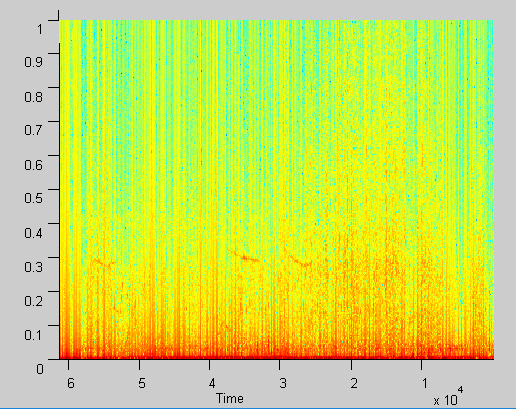
\includegraphics[width=.8\linewidth]{rumble_spectro.png}
  \caption{Spectrogram}
  \label{rumble_spectro}
\end{subfigure}%
\begin{subfigure}{.5\textwidth}
  \centering
  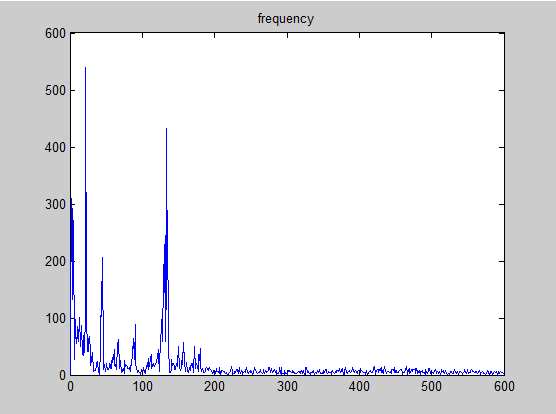
\includegraphics[width=.8\linewidth]{rumble_sfft.png}
  \caption{Frequency distribution}
  \label{fig:sub2}
\end{subfigure}
\caption[Spectrogram and the frequency distribution of a random rumble in the data set.]{Spectrogram and the frequency distribution of a random rumble in the data set. This shows how the samples are scattered in the infrasonic range and the visual pattern of the rumbles that we are looking for.}
\label{spectro:fft}
\end{figure} 

\paragraph{}
Pure rumbles were used for the initial training and the testing which consist 304 in number. Negative data set was generated from the background sound of recorded data in Yala, Kalawewa and other freely available infra sound recordings taken from the internet. 
\subsubsection{Training and testing}
\paragraph{}
104 positive and 110 negative samples were used for the training and 200 positive and 168 negative samples for the testing. That was 63\% of the total data set, which was used for the testing. Each data is processed as a 1 second windows without any overlap. Therefore, the input space is expanded according to the time duration of the audio clips. Each window is labeled according to the directory and fed into the SVM model.

\paragraph{}
For testing and evaluation, different performance measures were computed. The true positive percentage TP is the percentage of annotated rumbles detected as rumble, false positive percentage FP is the percentage of annotated rumbles detected as a negative or non-rumble, true negative percentage TN where annotated negative sound clips detected as negative, and false negative percentage FN is the percentage of annotated non rumbles detected as rumbles. Therefore, a test clip can fall in to TP, FP, TN or FN where more than 3 consecutive windows of the clip was classified. 3 is the rounded lowest mean time duration of all the rumble types in the data set in seconds. Given below is the mean time duration each type of elephant calls.

\begin{table}[H]
\centering
\begin{tabular}{|m{0.5\textwidth}|m{0.3\textwidth}|} 
\hline
\bf {Type of call} &  {\bf{Mean duration (s)}}\\
\hline
\hline
\bf {Bark-Rumbles} &  {\bf{ 3.7150}} \\
\hline
\bf {Chirp-Rumbles} &  {\bf{3.8933}} \\
\hline
\bf {Growls} &  {\bf{  4.7961}} \\
\hline
\bf {Long Roars} &  {\bf{ 3.3492}} \\
\hline
\bf {LongRoar-Rumbles} &  {\bf{4.4809}} \\
\hline
\bf {Rumbles} &  {\bf{ 5.4620}} \\
\hline
\bf {Roars} &  {\bf{ 2.2447}} \\
\hline
\bf {Roar-Rumbles} &  {\bf{3.8367}} \\
\hline
\end{tabular}
\end{table}
 
\subsubsection{Result and Evaluations}
\paragraph{}
After the first training, following results were obtained when we tested the detector for testing data set. 

\newpage
\begin{table}[H]
\centering
\begin{tabular}{|m{0.3\textwidth}|m{0.3\textwidth}|m{0.1\textwidth}|m{0.1\textwidth}|} 
\hline
\bf {File name} &  \bf{Out put vector} & \bf{Classified class} & \bf{Real class}\\
\hline
\bf {67132.wav} &  {\bf{[0 1 1 1 1 1 1 1]}} &  {\bf{1}} &  {\bf{1}} \\ \hline
\bf {35724.wav} &  {\bf{[0 1 1 1 1 1]}} &  {\bf{1}} &  {\bf{1}} \\ \hline
\bf {73776.wav} &  {\bf{[0 1 0 1 1 1 1 1 1 1 1 0]}} &  {\bf{1}} &  {\bf{1}} \\ \hline
\bf {87688.wav} &  {\bf{[0 1 1 1 1 1 1 1 1 1 1 1 1 1 1 1 1 1 0]}} &  {\bf{1}} &  {\bf{1}} \\ \hline
\bf {15448.wav} &  {\bf{[0 0 1 1 1 1 1 1 1 0]}} &  {\bf{1}} &  {\bf{1}} \\ \hline
\bf {62363.wav} &  {\bf{[0 1 1 1 1 1 1 1 0]}} &  {\bf{1}} &  {\bf{1}} \\ \hline
\bf {52035.wav} &  {\bf{[0 1 1 1 1 1 1]}} &  {\bf{1}} &  {\bf{1}} \\ \hline
\bf {22788.wav} &  {\bf{[0 1 1 1 1 1 1 1 1 1 1 1 0]}} &  {\bf{1}} &  {\bf{1}} \\ \hline
\bf {31031.wav} &  {\bf{[0 1 0 0 1]}} &  {\bf{0}} &  {\bf{1}} \\ \hline
\bf {42792.wav} &  {\bf{[0 0 1 1 1 0 1 1 1 1 1 0]}} &  {\bf{1}} &  {\bf{1}} \\ \hline
\bf {43122.wav} &  {\bf{[0 1 0 0 0 1 1 1 1 1 0]}} &  {\bf{1}} &  {\bf{1}} \\ \hline
\bf {96323.wav} &  {\bf{[0 1 1 1 1 1]}} &  {\bf{1}} &  {\bf{1}} \\ \hline
\bf {25676.wav} &  {\bf{[0 1 0 1 0 1 1 0]}} &  {\bf{0}} &  {\bf{1}} \\ \hline
\bf {01864.wav} &  {\bf{[0 0 0 0 1 0 0 0]}} &  {\bf{0}} &  {\bf{1}} \\ \hline
\bf {74175.wav} &  {\bf{[0 1 0 0 0 0 0 0 0 0 0 0 0 0 0]}} &  {\bf{0}} &  {\bf{1}} \\ \hline
\bf {69388.wav} &  {\bf{[0 1 1 1 1 1]}} &  {\bf{1}} &  {\bf{1}} \\ \hline
\bf {48967.wav} &  {\bf{[0 0 0 1 1 1 1 1 1 1 0]}} &  {\bf{1}} &  {\bf{1}} \\ \hline
\bf {36337.wav} &  {\bf{[0 1 0 0 0 0 1 0]}} &  {\bf{0}} &  {\bf{1}} \\ \hline
\bf {76703.wav} &  {\bf{[0 1 1 1 0]}} &  {\bf{}} &  {\bf{1}} \\ \hline
\bf {60033.wav} &  {\bf{[0 0 1 1 1 1 0]}} &  {\bf{1}} &  {\bf{1}} \\ \hline
\bf {49180.wav} &  {\bf{[0 1 1 1 1 1 1 1]}} &  {\bf{1}} &  {\bf{1}} \\ \hline
\bf {91912.wav} &  {\bf{[0 1 1 1 1 1 1 1 1 0]}} &  {\bf{1}} &  {\bf{1}} \\ \hline
\bf {rMice.wav} &  {\bf{[0 0 0 0 0 0 0 0 0 0 0]}} &  {\bf{0}} &  {\bf{1}} \\ \hline
\end{tabular}
\end{table}

\newpage
\paragraph{}
In the above table, randomly selected 23 clips from positive testing set are shown. In the first column, the file name of the clip is shown and in the second, each window output is shown in an array. '0' will indicate a negative class and '1' will indicate a positive class. In the third column, the overall classified class of the entire clip is shown considering 3 consecutive windows. In the last column, the real class label is shown. The table below shows some randomly selected clips from the testing set labeled as negative.

\begin{table}[H]
\centering
\begin{tabular}{|m{0.3\textwidth}|m{0.3\textwidth}|m{0.1\textwidth}|m{0.1\textwidth}|} 
\hline
\bf {File name} &  \bf{Out put vector} & \bf{Classified class} & \bf{Real class}\\
\hline
\bf {Neg29.wav} &  {\bf{[0 0 0 0 0 0 0 0 0 0 0 0 0 0 0 0 0 0 0]}} &  {\bf{0}} &  {\bf{0}} \\ \hline
\bf {Neg3.wav} &  {\bf{[0 0 0 0 0 0 0 0 0 0 0 0 0]}} &  {\bf{0}} &  {\bf{0}} \\ \hline
\bf {Neg30.wav} &  {\bf{[0 0 0 0 0 0 0 0 0 0 0 0 0 0 0 0 0 0 0 0]}} &  {\bf{0}} &  {\bf{0}} \\ \hline
\bf {Neg31.wav} &  {\bf{[0 0 0 0 0 0 0 0 0 0 0 0 0 0 0]}} &  {\bf{0}} &  {\bf{0}} \\ \hline
\bf {Neg32.wav} &  {\bf{[0 0 0 0 0 0 0 0 0 0 0 0 0 0 0 0 0]}} &  {\bf{0}} &  {\bf{0}} \\ \hline
\bf {Neg33.wav} &  {\bf{[0 0 0 0 0 0 0 0 0 0 0 0 0 0 0 0 0]}} &  {\bf{0}} &  {\bf{0}} \\ \hline
\bf {Neg34.wav} &  {\bf{[0 1 1 1 1 0 1 0 0 1]}} &  {\bf{1}} &  {\bf{0}} \\ \hline
\bf {Neg35.wav} &  {\bf{[0 0 0 0 0 0 0 0 0 0 0 0 0 0 0 0]}} &  {\bf{0}} &  {\bf{0}} \\ \hline
\bf {Neg16.wav} &  {\bf{[0 0 0 0 0 0 0 0 0 0 0 0 0 0 0 0]}} &  {\bf{0}} &  {\bf{0}} \\ \hline
\bf {Neg17.wav} &  {\bf{[0 0 0 0 0 0 0 0 0 0 0 0 0 0 0]}} &  {\bf{0}} &  {\bf{0}} \\ \hline
\bf {Neg18.wav} &  {\bf{[0 0 0 0 0 0 0 0 0 0 0 0 0 0 0 0]}} &  {\bf{0}} &  {\bf{0}} \\ \hline
\bf {Neg19.wav} &  {\bf{[0 0 0 0 0 0 0 0 0 0 0 0 0 0]}} &  {\bf{0}} &  {\bf{0}} \\ \hline
\bf {Neg2.wav} &  {\bf{[0 1 1 0 0]}} &  {\bf{1}} &  {\bf{0}} \\ \hline

\end{tabular}
\end{table}

\paragraph{}
Given above show only some randomly selected data to provide an overview of the classification process and the following table shows a summary using the evaluation parameters for the whole initial experimental classification.
\begin{table}[H]
\centering
\begin{tabular}{|m{0.5\textwidth}|m{0.3\textwidth}|} 
\hline
\bf {Performance measure} &  {\bf{Percentage}}\\
\hline
\hline
\bf {True Positive (TP)} &  {\bf{89.96}} \\
\hline
\bf {False Positive (FP)} &  {\bf{10.04}} \\
\hline
\bf {True Negative (TN)} &  {\bf{89.41}} \\
\hline
\bf {False Negative (FN)} &  {\bf{10.58}} \\
\hline
\end{tabular}
\end{table}


\paragraph{}
After the initial experimental training and testing using raw rumble and negative data, the signal enhancement method proposed in \cite{11} and explained in the Methodology chapter was applied and the training process was repeated. This was done for the same data set that was used initially. Given below is the summary of experiment two after applying the signal enhancement.
\begin{table}[H]
\centering
\begin{tabular}{|m{0.5\textwidth}|m{0.3\textwidth}|} 
\hline
\bf {Performance measure} &  {\bf{Percentage}}\\
\hline
\hline
\bf {True Positive (TP)} &  {\bf{95.78}} \\
\hline
\bf {False Positive (FP)} &  {\bf{4.22}} \\
\hline
\bf {True Negative (TN)} &  {\bf{93.65}} \\
\hline
\bf {False Negative (FN)} &  {\bf{4.23}} \\
\hline
\end{tabular}
\end{table}

\paragraph{}
As we can see in the results of the second experiment, results after signal enhancement clearly outperforms the results of the first experiment. The true positive and true negative percentages have increased while the false classification parameters have decreased. Both methods employ the modified MFCC features introduced in Chapter 3, which use a frequency range from 0 to 300 Hz. Although the infrasonic range is between 0 Hz to 20hz, we observe that rumbles frequently exceed this frequency range due to the harmonics. Therefore, taking the upper limit as 300Hz has had a high impact on the accuracy of detection. We observed a reduction in accuracy when this range is decreased. 


\newpage
\section{Conclusion and Future Works.}
\subsection{Conclusion}
\paragraph{}
Throughout this research we were able to achieve our two objectives up to a certain extent with some tradeoffs came across in the practical environments. Though this is only the initial step of an elephant early warning system, the result of this research will make a motivation for the future works. Experiments we conducted fall into study on either localization or pattern recognition.

\paragraph{}
Significance of the localization result is that the angles with that much of accuracy was achieved by the laboratory made, low cost Elocate sensors specially designed to capture infra sound. Although the localization is deriving the distance and the angle of a particular location from another, we have only estimated the angle. When the real location is calculated from the angles geometrically, error from each angle will be propagated. This will cause distance to have large errors. This should be separately addressed by using more Elocate nodes or applying an error correction mechanism. 
We were able to localize from 400m away maximum due to the limitations in the university premises. We monitored that when the angle is getting closer to 0\textsuperscript{o} the indented error. This indicates that we can reliably use an angle value calculated using a pair of Eloc nodes if the angle to the infrasonic source is greater than approximately 30\textsuperscript{o} degrees. By using multiple pairs of Eloc nodes deployed at different angles to each other, we can select the most reliable node pairs for the final location by ignoring the ones which measure an angle less than 30\textsuperscript{o} degrees to the infrasonic source. 

\paragraph{}
Recordings we did in the wild was extremely beneficial when training the detector and confirming the performance of the Elocate node. A zoologist was able to detect elephant rumbles in the sound recordings that we have done in the wild with
Eloc nodes, thus establishing their effectiveness in capturing elephant infrasonic calls. However this is the first attempt of implementing an Asian elephant detector using infra sound. This research has proved that a rumble of an Asian elephant could be detected automatically by analyzing its acoustic features, with an impressive level of accuracy. One drawback is when this is going to be deployed in the real environment is that this model was trained only for rumbles but an elephant emit vast varieties of calls such as trumpets barks and etc. And also in this research we have used MFCC for feature extraction which is designed to process human vocals. This model will have a higher accuracy if a more generalized method such as Green Wood filter was used. For the application of the proposed method as an early warning system the accuracy needed to be improved further by doing a principle component analysis to figure out the most suitable spectral features.   

\subsection{Future Works} 
\paragraph{}
Since this is an initial step to a system that can detect and localize Asian elephants, this has opened many doors for some other possibilities. One of them is to study on distance estimation of infra sound to from receiver to sender employing the localized angles. And also experimenting to estimate angles from longer distance also a future work.
The training model neededs to be tested for large data set recorded from Elocate sensors, where we tested mostly for the data set recorded from an advanced and dedicated device for animal sound recording.  

\paragraph{}
Most challenging work ahead is deploying this system in the real world. Localization and detection should be optimized to be run in low cost and low performing hardware devices like Arduino, Raspberry pi and etc. The main challenge we come across is the lack of 3G/4G internet connectivity in the villages bounded to the forests. Therefore the communication between devices should be very minimum. Theses findings will impact on the betterment of humen and elephant if a real elephant detector and localizer is deployed in the real world. 

\newpage
\appendix
\section{Appendix}
\begin{lstlisting}[language=Matlab]
% Copyright (c) 2016, Matthias Zeppelzauer
% 
% All rights reserved.
% 
% Redistribution and use in source and binary forms, with or without
% modification, are permitted provided that the following conditions are met:
% 1. Redistributions of source code must retain the above copyright
%    notice, this list of conditions and the following disclaimer.
% 2. Redistributions in binary form must reproduce the above copyright
%    notice, this list of conditions and the following disclaimer in the
%    documentation and/or other materials provided with the distribution.
% 3. All advertising materials mentioning features or use of this software
%    must display the following acknowledgement:
%    This product includes software developed by the <organization>.
% 4. Neither the name of the <organization> nor the
%    names of its contributors may be used to endorse or promote products
%    derived from this software without specific prior written permission.
% 
% THIS SOFTWARE IS PROVIDED BY MATTHIAS ZEPPELZAUER ''AS IS'' AND ANY
% EXPRESS OR IMPLIED WARRANTIES, INCLUDING, BUT NOT LIMITED TO, THE IMPLIED
% WARRANTIES OF MERCHANTABILITY AND FITNESS FOR A PARTICULAR PURPOSE ARE
% DISCLAIMED. IN NO EVENT SHALL MATTHIAS ZEPPELZAUER BE LIABLE FOR ANY
% DIRECT, INDIRECT, INCIDENTAL, SPECIAL, EXEMPLARY, OR CONSEQUENTIAL DAMAGES
% (INCLUDING, BUT NOT LIMITED TO, PROCUREMENT OF SUBSTITUTE GOODS OR SERVICES;
% LOSS OF USE, DATA, OR PROFITS; OR BUSINESS INTERRUPTION) HOWEVER CAUSED AND
% ON ANY THEORY OF LIABILITY, WHETHER IN CONTRACT, STRICT LIABILITY, OR TORT
% (INCLUDING NEGLIGENCE OR OTHERWISE) ARISING IN ANY WAY OUT OF THE USE OF THIS
% SOFTWARE, EVEN IF ADVISED OF THE POSSIBILITY OF SUCH DAMAGE.
% 
% 
% Perform sound enhancement by the application of the 2D tensor on the spectrogram
%
% Inputs: - an audio spectrogram
% 		  - the size of a 2-dimensional Gaussian filter, e.g. [15 20], to smooth the output
%
% Outputs: - l1, l2: the two eigenvalues for each pixel in the spectrogram
%		   - coherence: the coherence computed from the eigenvalues  
%		   - discriminant: the discriminant computed from the eigenvalues 
%		   - sumEV: the sum of the eigenvalues 
%		   - prodEV: the product of the eigenvalues 
%		   - coherence: the coherence computed from the eigenvalues  	
%		   - Gx, Gy: the temporal and spatial gradient from the spectrogram (for each pixel) 		
%
% If you use this code, please cite this paper:
% 	Zeppelzauer, M., Stöger, A. S., & Breiteneder, C. (2013, October). 
% 	Acoustic detection of elephant presence in noisy environments. 
% 	In Proceedings of the 2nd ACM international workshop on Multimedia 
% 	analysis for ecological data (pp. 3-8). ACM.


function [l1, l2, coherence, discriminant, sumEV, prodEV, Gx, Gy] = computeTensor(spec,gaussWinSize)

[Ix, Iy]=gradient(spec);

%get tensor
Ix2 = Ix.*Ix;
Iy2 = Iy.*Iy;
Ixy = Ix.*Iy;



filt = fspecial('gaussian',gaussWinSize,sqrt(prod(gaussWinSize))/4); 
%figure; mesh(filt)
Gx = Ix;
Gy = Iy;
Gx = conv2(Ix,filt,'same');
Gy = conv2(Iy,filt,'same');



%filter tensor by gaussian
Ix2 = conv2(Ix2,filt,'same');
Iy2 = conv2(Iy2,filt,'same');
Ixy = conv2(Ixy,filt,'same');

%compute eigenvalues
l1 = 0.5*((Ix2 + Iy2) + sqrt( (Ix2-Iy2).^2 + 4*Ixy.^2)); 
l2 = 0.5*((Ix2 + Iy2) - sqrt( (Ix2-Iy2).^2 + 4*Ixy.^2)); 

discriminant = Ix2 .* Iy2 - Ixy.^2 + (Ix2 + Iy2).^2; %Formula: det(T)+trace(T)^2
sumEV = Ix2 + Iy2; %indicator for edges and cordners
prodEV = Ix2 .* Iy2 - Ixy.^2; %indicator for edges and cordners
coherence = ((l1-l2)./(l1+l2)).^2;


\end{lstlisting}
\newpage
\begin{thebibliography}{1}
\bibitem{13} \emph{ Lalith Seneviratne, G. Rossel, W.D.C.. Gunasekera, H.L.P.A. Madanayake, Y.M.S.S. Yapa and G. Doluweera.Elephant Infrasound Calls as a Method for Electronic Elephant Detection.}
\bibitem{5} Szabo T. L., 1994, “Time domain wave equations for lossy media obeying a frequency power law,” J. Acoust. Soc. Am., 96(1), pp. 491-500.
\bibitem{28}M.P.J. Dharmaratne and P.C. Magedaragamage, Human-Elephant conflict and solutions to it in Sri Lanka.
\bibitem{28.5} W. AREAS and R. Shunmugam, "Human - elephant conflict,". [Online]. Available: http://wwf.panda.org/whatwedo/endangeredspecies/elephants/humanelephantconflict.cfm. Accessed: Jan. 2, 2017.
\bibitem{1} \emph{Berg, J.K. 1983. Vocalizations and associated behaviours of the African elephant Loxodonta africana in captivity. Z. Tierpsychol 63:63-79.}
\bibitem{2}Payne, K. 2003. Sources of Social Complexity in the Three Elephant Species. In: Animal Social Complexity: Intelligence, Culture, and Individualized Societies. Ed: Frans B.M. de Waal and Peter L. Tyack. Harvard University Press.
\bibitem{12} MUSIC Algorithm", Ptolemy.eecs.berkeley.edu, 2016. [Online]. Available: http://ptolemy.eecs.berkeley.edu/papers/96/dtmf\_ict/www/node5.html. [Accessed: 27- Apr- 2016].
\bibitem{3} Payne, K., Langbauer, Jr., W.R., and Thomas, E. 1986. Infrasonic calls of the Asian elephant (Elephas maximus). Behavioral Ecology and Sociobiology.
\bibitem{4} “Infrasonic Sound", Hyperphysics.phyastr.gsu.edu, 2016. [Online]. Available: http://hyperphysics.phy-astr.gsu.edu/hbase/sound/infrasound.html. [Accessed: 27- Apr- 2016].
\bibitem{14} J. E. Piercy, T. F. W. Embleton, L. C. Sutherland, Review of noise propagation in the atmosphere, J. Acoust. Soc. Am. Volume 61, Issue 6, pp. 1403-1418, June 1977.
\bibitem{10} P. J. Venter and J. J. Hanekom. Automatic detection of african elephant (loxodonta africana) infrasonic vocalisations from recordings. Biosystems engineering.
\bibitem{15} Panasonic Corporation. Panasonic Omnidirectional Back Electret Condenser Microphone Cartidge.[2016].  [Online]. Available: http://industrial.panasonic.com/cdbs/www-data/pdf/ABA5000/ABA5000CE22.pdf. [Accessed: 28- Apr- 2016].
\bibitem{16}"LM358 | General Purpose Amplifier | Operational Amplifier (Op Amp) | Description \& parametrics", Ti.com, 2016. [Online]. Available: http://www.ti.com/product/LM358. [Accessed: 28- Apr- 2016].
\bibitem{17}Jean-Marc Valin, Franc¸ois Michaud, Jean Rouat, Dominic Letourneau LABORIUS - Research Laboratory on Mobile Robotics and Intelligent Systems Department of Electrical Engineering and Computer Engineering Universite´ de Sherbrooke.Robust Sound Source Localization Using a Microphone Array on a Mobile Robot.
\bibitem{18} Richard F. Lyon, Andreas G. Katsiamis, Emmanuel M. Drakakis (2010). "History and Future of Auditory Filter Models"
\bibitem{19} Shermin de Silva "Acoustic communication in the Asian elephant,
Elephas maximus maximus"
\bibitem{20} Taff, L. G, “Target Localization from Bearings-only Observations,”
IEEE Trans. Aerosp. Electron., 3, issue 1, (1997).New York: McGraw-Hill, 1964, pp. 15–64.
\bibitem{21}D.Li, and Y. H. Hu, “Energy Based Collaborative Source Localization
Using Acoustic Micro-Sensor Array,” EURASIP Journal on Applied
Signal Processing, vol. 2003, no. 4, pp. 321-337, 2003.
\bibitem{22}M. Brandstein and H. Silverman, “A Practical Methodology for Speech
Source Localization with Microphone arrays,” Comput., Speech Lng.,
vol. 11, no. 2, pp. 91-126, 1997.
\bibitem{23} G. C. Carter, “Tutorial Overview of Coherence and Time Delay Estimation,”
in Coherence and Time Delay Estimation—An Applied Tutorial for Research, Development, Test, and Evaluation Engineers, vol. 1,1993,pp. 1–27
\bibitem{24}C. H. Knapp and G. C. Carter, “The Generalized Correlation Method for Estimation of Time Delay,” IEEE Trans. Acoust., Speech, Signal Processing,vol. ASSP-24, pp. 320–327, Aug.1976.
\bibitem{6} Payne, K., Thompson, M., and Kramer, L. 2003. Elephant calling patterns as indicators of group size and composition: the basis for an acoustic monitoring system. African Journal of Ecology, 41: 99-107
\bibitem{7} "INFILTEC: The Inexpensive Infrasound Monitor Project. - simple microbarograph design for DIY", Infiltec.com, 2016. [Online]. Available: http://www.infiltec.com/Infrasound@home/. [Accessed: 27- Apr- 2016].
\bibitem{8} A. Vedurmudi, J. Goulet, J. Christensen-Dalsgaard, B. Young, R. Williams and J. van Hemmen, "How Internally Coupled Ears Generate Temporal and Amplitude Cues for Sound Localization",Phys. Rev. Lett., vol. 116, no. 2, 2016.
\bibitem{9} ] Larom, D., M. Garstang, K. Payne, R. Raspet \& M. Lindeque. 1997. The influence of surface atmospheric conditions on the range and area reached by animal vocalizations. J. Experimental Biol. 200: 421-431.

\bibitem{11} Acoustic Detection of Elephant Presence in Noisy Environments Matthias Zeppelzauer Vienna University of Technology.



\bibitem{25}  J.benesty, “Adaptive Eigenvalue Decomposition Algorithm for Passive Acoustic Source Localization,” Acoustical Society of America, January 2000.
\bibitem{26} Hasan Khaddour, "A Comparison of Algorithms of Sound Source Localization Based
on Time Delay Estimation"
\bibitem{27} Sasha Devore,Antje Ihlefeld,Kenneth Hancock,Barbara Shinn-Cunningham,Bertrand Delgutte,
"Accurate Sound Localization in Reverberant Environments Is Mediated by Robust Encoding of Spatial Cues in the Auditory Midbrain"
\bibitem{29} Infiltec Model INFRA-20 the inexpensive infrasound monitor device. http://www.infiltec.com/Infrasound@home/. Accessed: 2015-07-29.
\bibitem{30} K. B. Payne, J. W. R. Langbauer, and E. M. Thomas. Infrasonic calls of the asian elephant (elephas maximus). Behavioral Ecology and Sociobiology, 18(4):297–301, 1986.
\bibitem{31}P. Dabare, C. Suduwella, A. Sayakkara, D. Sandaruwan, C. Keppitiyagama, K. De Zoysa, K. Hewage, and T. Voigt. Listening to the giants: Using elephant infra-sound to solve the human-elephant conflict. In Proceedings of the 6th ACMWorkshop on RealWorldWireless Sensor Networks, pages 23–26. ACM, 2015.
\bibitem{32} S. Blake, I. Douglas-Hamilton, andW. Karesh. Gps telemetry of forest elephants in central africa: results of a preliminary study. African Journal of Ecology, 39(2):178–186, 2001.
\bibitem{33}H. Wang, C.-E. Chen, A. Ali, S. Asgari, R. E. Hudson, K. Yao, D. Estrin, and C. Taylor. Acoustic sensor networks for woodpecker localization. In Optics Photonics 2005, pages 591009–591009. International Society for Optics and Photonics, 2005.
\bibitem{34}Y.-E. Kim, C.-H. Jeon, D.-H. Su, J.-K. Lee, J.-G. Chung, and K.-J. Cho. Sound Source Localization Method Using Region Selection.INTECH Open Access Publisher, 2011.
\bibitem{35}J. Taylor. Introduction to Error Analysis, the Study of Uncertainties in Physical Measurements, 2nd Edition. University Science Books, Aug.1997.
\bibitem {36} Davis, S. Mermelstein, P. (1980) Comparison of Parametric Representations for Monosyllabic Word Recognition in Continuously Spoken Sentences. In IEEE Transactions on Acoustics, Speech, and Signal Processing, Vol. 28 No. 4, pp. 357-366
\bibitem {37} P. J. Clemins, M. B. Trawicki, K. Adi, J. Tao, and M. T. Johnson. Generalized perceptual features for
vocalization analysis across multiple species. In Proc. of the IEEE Int. Conf. on Acoustics, Speech and Signal Proc., volume 1, pages 253–256, 2006.
\bibitem {38} C. Harris and M. Stephens. A combined corner and edge detector. In 4th Alvey vision conference.
\bibitem {39}  Andrey Temko*, Climent Nadeu, Classification of acoustic events using SVM based clustering schemes.
\bibitem {40} G. Guo, Z. Li, "Content-based Audio Classification and Retrieval using Support Vector Machines", IEEE
Transactions on Neural Networks, vol. 14, pp 209-215, January, 2003.
\bibitem {41} Machine Learning Mastery. 2016. A Gentle Introduction to Scikit-Learn. [ONLINE] Available at: http://machinelearningmastery.com/a-gentle-introduction-to-scikit-learn-a-python-machine-learning-library/. 
\bibitem {42} C. U. Barcus, "What elephant calls mean," National Geographic. [Online]. Available: http://www.nationalgeographic.com/news-features/what-elephant-calls-mean/. Accessed: Jan. 1, 2017.

\end{thebibliography}

\end{document}